%%
%% This is file `sample-authordraft.tex',
%% generated with the docstrip utility.
%%
%% The original source files were:
%%
%% samples.dtx  (with options: `authordraft')
%% 
%% IMPORTANT NOTICE:
%% 
%% For the copyright see the source file.
%% 
%% Any modified versions of this file must be renamed
%% with new filenames distinct from sample-authordraft.tex.
%% 
%% For distribution of the original source see the terms
%% for copying and modification in the file samples.dtx.
%% 
%% This generated file may be distributed as long as the
%% original source files, as listed above, are part of the
%% same distribution. (The sources need not necessarily be
%% in the same archive or directory.)
%%
%% The first command in your LaTeX source must be the \documentclass command.
\documentclass[sigconf]{acmart}
%% NOTE that a single column version may required for 
%% submission and peer review. This can be done by changing
%% the \doucmentclass[...]{acmart} in this template to 
%% \documentclass[manuscript,screen]{acmart}
%% 
%% To ensure 100% compatibility, please check the white list of
%% approved LaTeX packages to be used with the Master Article Template at
%% https://www.acm.org/publications/taps/whitelist-of-latex-packages 
%% before creating your document. The white list page provides 
%% information on how to submit additional LaTeX packages for 
%% review and adoption.
%% Fonts used in the template cannot be substituted; margin 
%% adjustments are not allowed.

\usepackage{multirow}
\usepackage{subcaption}
\usepackage{algorithm}
\usepackage[noend]{algpseudocode}
\setcopyright{rightsretained}
%%
%% \BibTeX command to typeset BibTeX logo in the docs
\AtBeginDocument{%
  \providecommand\BibTeX{{%
    \normalfont B\kern-0.5em{\scshape i\kern-0.25em b}\kern-0.8em\TeX}}}

%% Rights management information.  This information is sent to you
%% when you complete the rights form.  These commands have SAMPLE
%% values in them; it is your responsibility as an author to replace
%% the commands and values with those provided to you when you
%% complete the rights form.
\setcopyright{acmcopyright}
\copyrightyear{2022}
\acmYear{2022}
\acmDOI{XXXXXXX.XXXXXXX}

%% These commands are for a PROCEEDINGS abstract or paper.
\acmConference[e-Energy '22]{Thirteenth ACM International Conference on Future Energy Systems}{Jun 28 - Jul 1, 2022}{Virtual}
\acmBooktitle{e-Energy '22: Thirteenth ACM International Conference on Future Energy Systems,
  Jun 28 - Jul 1, 2022, Virtual}
\acmPrice{15.00}
\acmISBN{123-4-4567-XXXX-X/18/06}
%
%  Uncomment \acmBooktitle if th title of the proceedings is different
%  from ``Proceedings of ...''!
%
%\acmBooktitle{Woodstock '18: ACM Symposium on Neural Gaze Detection,
%  June 03--05, 2018, Woodstock, NY} 
\acmPrice{15.00}
\acmISBN{978-1-4503-XXXX-X/18/06}


%%
%% Submission ID.
%% Use this when submitting an article to a sponsored event. You'll
%% receive a unique submission ID from the organizers
%% of the event, and this ID should be used as the parameter to this command.
%%\acmSubmissionID{123-A56-BU3}

%%
%% The majority of ACM publications use numbered citations and
%% references.  The command \citestyle{authoryear} switches to the
%% "author year" style.
%%
%% If you are preparing content for an event
%% sponsored by ACM SIGGRAPH, you must use the "author year" style of
%% citations and references.
%% Uncommenting
%% the next command will enable that style.
% \citestyle{acmauthoryear}



% \author{Paper: \#100}
% \affiliation{%
%   \institution{}
%   \city{ }
%   \country{ }}




%%
%% end of the preamble, start of the body of the document source.
\begin{document}

%%
%% The "title" command has an optional parameter,
%% allowing the author to define a "short title" to be used in page headers.
\title{Poster: A Realistic Dataset Generator for Smart Grid Ecosystems with Electric Vehicles}

%%
%% The "author" command and its associated commands are used to define
%% the authors and their affiliations.
%% Of note is the shared affiliation of the first two authors, and the
%% "authornote" and "authornotemark" commands
%% used to denote shared contribution to the research.

\author{Georgios Charalambidis}
% \authornote{Both authors contributed equally to this research.}
% \email{trovato@corporation.com}
% \orcid{1234-5678-9012}
% \author{G.K.M. Tobin}
% \authornotemark[1]
% \email{webmaster@marysville-ohio.com}
\affiliation{%
  \institution{School of Electrical \& Computer Engineering}
%   \streetaddress{P.O. Box 1212}
%   \city{Dublin}
%   \state{Ohio}
   \country{Technical University of Crete, Greece}
%   \postcode{43017-6221}
}
\email{gcharalampidis@isc.tuc.gr}
\author{Charilaos Akasiadis}
\affiliation{%
  \institution{Institute of Informatics \& Telecommunications}
%   \streetaddress{1 Th{\o}rv{\"a}ld Circle}
%   \city{Hekla}
  \country{NCSR ``Demokritos'', Greece}
}
\email{cakasiadis@iit.demokritos.gr}

% \email{larst@affiliation.org}
\author{Emmanouil S. Rigas}
\affiliation{%
  \institution{School of Medicine}
%   \city{Rocquencourt}
  \country{Aristotle University of Thessaloniki, Greece}
}
\email{erigas@auth.gr}

\author{Georgios Chalkiadakis}
\affiliation{%
 \institution{School of Electrical \& Computer Engineering}
%  \streetaddress{Rono-Hills}
%  \city{Doimukh}
%  \state{Arunachal Pradesh}
 \country{Technical University of Crete, Greece}
}
 \email{gehalk@intelligence.tuc.gr}

% \author{Huifen Chan}
% \affiliation{%
%   \institution{Tsinghua University}
%   \streetaddress{30 Shuangqing Rd}
%   \city{Haidian Qu}
%   \state{Beijing Shi}
%   \country{China}}

% \author{Charles Palmer}
% \affiliation{%
%   \institution{Palmer Research Laboratories}
%   \streetaddress{8600 Datapoint Drive}
%   \city{San Antonio}
%   \state{Texas}
%   \country{USA}
%   \postcode{78229}}
% \email{cpalmer@prl.com}

% \author{John Smith}
% \affiliation{%
%   \institution{The Th{\o}rv{\"a}ld Group}
%   \streetaddress{1 Th{\o}rv{\"a}ld Circle}
%   \city{Hekla}
%   \country{Iceland}}
% \email{jsmith@affiliation.org}

% \author{Julius P. Kumquat}
% \affiliation{%
%   \institution{The Kumquat Consortium}
%   \city{New York}
%   \country{USA}}
% \email{jpkumquat@consortium.net}

%%
%% By default, the full list of authors will be used in the page
%% headers. Often, this list is too long, and will overlap
%% other information printed in the page headers. This command allows
%% the author to define a more concise list
%% of authors' names for this purpose.
\renewcommand{\shortauthors}{G. Charalambidis, et al.}

%%
%% The abstract is a short summary of the work to be presented in the
%% article.
\begin{abstract}

%The widespread use of electric mobility technologies such as the Electric Vehicles (EVs), poses certain challenges both from the technical, and the socioeconomic points of view. 
%In order to address these, research must utilize related data that originates from realistic sources.
%However, in the typical case, such data contains private and sensitive information that cannot be made available to the researchers. As a result, research makes use of the few datasets that are publicly available. At the same time, the majority of the available data, contain only a few customers, while hundreds of thousands are required. To overcome such obstacles, synthetic data can be used, which nevertheless originates from models with relationships that sufficiently capture the properties of the actual real-world datasets.
Research on the deployment and employment of electric vehicles (EVs) in the emerging Smart Grid, typically requires access to large datasets containing data that is rich and reliable. Such datasets are hard to come by in the wild due to various privacy and sensitivity considerations.
In this paper, we design a dataset generator for large-scale EVs charging management. The generator {\em (i)} takes as input anonymized real-world datasets 
%, which however is possibly inconsistent and overused, 
describing 
different energy generation and demand types, as well as charging profiles of EVs and corresponding trip and type information; {\em (ii)} fits a variety of machine learning models using this data as training sets; and {\em (iii)} generates new synthetic data that adheres to the same principles and relationships as the input.
The generator comes complete with data smoothing and dataset summarization, visualization, and comparison abilities that users can utilize via a web-based interface; and is offered as a free-to-use tool to the research community. %via an online repository.
%respective summarizations, which includes barplots and histograms to visualize the results, and different metrics in order to quantify a ‘distance’ between the distributions under comparison. These summarizations give us a complete picture of the generated data and they are particularly useful for detecting correspondence issues. Last but not least, the dataset generator is available via an online repository and it can readily be incorporated by third parties in their research processes.
\end{abstract}


\begin{CCSXML}
<ccs2012>
<concept>
<concept_id>10010147.10010341.10010349.10010363</concept_id>
<concept_desc>Computing methodologies~Data assimilation</concept_desc>
<concept_significance>300</concept_significance>
</concept>
</ccs2012>
\end{CCSXML}

\ccsdesc[300]{Computing methodologies~Data assimilation}
%%
%% Keywords. The author(s) should pick words that accurately describe
%% the work being presented. Separate the keywords with commas.
\keywords{Dataset Generator, Electric Vehicles, Charging, Smart Grid}

%% A "teaser" image appears between the author and affiliation
%% information and the body of the document, and typically spans the
%% page.
% \begin{teaserfigure}
%   \includegraphics[width=\textwidth]{sampleteaser}
%   \caption{Seattle Mariners at Spring Training, 2010.}
%   \Description{Enjoying the baseball game from the third-base
%   seats. Ichiro Suzuki preparing to bat.}
%   \label{fig:teaser}
% \end{teaserfigure}

%%
%% This command processes the author and affiliation and title
%% information and builds the first part of the formatted document.
\acmYear{2022}\copyrightyear{2022}
\acmConference[e-Energy '22]{The Thirteenth ACM International Conference on Future Energy Systems}{June 28--July 1, 2022}{Virtual Event, USA}
\acmBooktitle{The Thirteenth ACM International Conference on Future Energy Systems (e-Energy '22), June 28--July 1, 2022, Virtual Event, USA}
\acmPrice{15.00}
\acmDOI{10.1145/3538637.3538755}
\acmISBN{978-1-4503-9397-3/22/06}

\maketitle

%%%%%%%%%%%%%%%%%%%%%%%%%%%%%%%%%%%%%%%%%%%%%%%%%%%%%%%%%%%%%%%%%%%%%%%%%%%%%%%%%%%%%%
\section{Introduction}
% Climate change is driving a transition towards less fossil fuel- consuming processes and sustainable societies. The important sector of mobility is currently facing a transformation where Electric Vehicles (EVs) are promoted as an alternative to reduce pollution; due to the absence of direct emissions during operation, EVs are a promising technology that offers practical reductions of the $CO_2$ emissions. This of course only holds, provided that the additional energy that fulfills the increased demand originating from EVs is produced by renewable sources.

Although EV deployment has been growing rapidly over the past ten years, many challenges still arise in different levels. 
For instance, the charging infrastructure needs to be properly placed to service large numbers of customers \cite{xiong2021electric}; a variety of critical elements of vehicle-to-grid (V2G) economics have to be accurately identified and confronted~\cite{steward2017critical}; while there is a need for the appropriate re-design of the electricity distribution network to accomodate EVs~\cite{flammini2017interaction}
As such, there is an utmost need for reliable data for a variety of purposes---e.g., for  understanding behaviors, exploring flexibility, and extrapolating results for other similar cases or sites. However, the lack of reliable data to advance this highly interdisciplinary research, is a known problem in this rising market~\cite{pevec2019electric}. Even 
%where efforts have been made to make 
when datasets are publicly available~\cite{barker2012smart,pecan}, limitations still arise---e.g., the range/size of the %public 
datasets is limited, or the data available may be subject to copyright and not freely shared for use.
% while a grand challenge indeed arises for AI and MAS research \cite{kamboj2011deploying}, which is assigned the task, among others to optimize G2V/V2G operations, while respecting various interoperability and privacy issues~\cite{ramchurn2012putting, tao2017foud}. 

This %fact 
calls for simulators to address data engineering needs and enable the design and analysis of novel components with minimum risk.
% and the global stock of EV passenger vehicles passed 5 million in 2018, with an increase of 63\% since 2017, while the rising trend continues ~\cite{newell2019global}. %Successfully establishing electric mobility solutions and maximizing the technological advantage from a societal aspect, requires a multilevel approach that involves car manufacturers and owners, building and civil infrastructure managers, and power system authorities to collaborate.
% EVs are envisaged to operate within 
% %the so-called 
% the emerging Smart Grid, which is equipped with algorithms that have the ability to efficiently manage large numbers of EVs~\cite{7000557,ramchurn2012putting}, allowing the conduction of key Grid-to-Vehicle (G2V)  \cite{valogianni2015multiagent,hayakawa2015online, gerding2011online, 10.1145/3396851.3397727} and Vehicle-to-Grid (V2G)  \cite{kempton2005vehicle} tasks in a large scale.
%The EVs' operation is two-folded: On the one hand, they can charge their batteries, preferably using energy from renewable sources, %that are characterized by high intermittency, 
%operating in a Grid-to-Vehicle (G2V) mode \cite{valogianni2015multiagent,hayakawa2015online, gerding2011online}. On the other hand, they can discharge their batteries, effectively operating as temporal storage devices \cite{lund2008integration} in a Vehicle-to-Grid (V2G) mode \cite{kempton2005vehicle}, thus significantly increasing the storage capacity of the 
%electricity 
%network and reducing the energy that is wasted when the demand is lower than the supply. 
%In both cases
%, the vehicles need  both in the G2V \cite{hayakawa2015online, gerding2011online} and the V2G \cite{koufakis2019offline} operation of the EVs.
% However, to that end, many challenges still arise in different levels, including the technical and financial ones. For instance, huge challenges lie ahead for the operation and design of the electricity distribution network~\cite{flammini2017interaction}; the charging infrastructure needs to be properly placed to service large numbers of customers \cite{xiong2021electric}; a variety of critical elements of vehicle-to-grid economics have to be accurately identified and dealt with~\cite{steward2017critical}; while a grand challenge indeed arises for artificial intelligence and multiagent systems research \cite{kamboj2011deploying}, which is assigned the task, among others to optimize the aforementioned G2V/V2G operations, while respecting various interoperability and privacy issues~\cite{ramchurn2012putting, tao2017foud}. As such, there is a profound need for thorough interdisciplinary research in this rising market. This in turn calls for efficient and effective simulators, to address data engineering needs and enable the design and analysis of novel components with minimum technical or financial risk.
% Now, data collected from smart grid ecosystems as well as from electric vehicles can be used for both academic and industrial purposes. Increased data input has been a major concern in the energy informatics sector over the last decade~\cite{watson2010information}. Previous studies of different EV datasets include statistical analysis of data collected in the Netherlands by ElaadNL~\cite{develder2016quantifying,quiros2018statistical} and analysis of EV energy consumption based on data collected by the US Department of Energy~\cite{islam2018extensive}. 
%These 
Lee et al.~\cite{lee2019acnDATA} introduced ACN-Data, a dynamically populated dataset of EVs charging in workplaces, which, however, only includes workplace EV charging data, but no trips-related or production and consumption data. 
% This is also the case for the work of~\cite{amara2021review}, where a review of available EV charging data is included.
RAMP-mobility~\cite{MANGIPINTO2022118676}, relies on user input that indicates specific properties of the data
% (e.g., population characteristics or peak intervals duration), 
and generates mobility and demand data for a number of EVs, using a stochastic model.
EMOBPY~\cite{gaete2021open}, %receives in the input 
employs relative frequencies calculated using real data to generate time series of vehicle mobility, %driving 
energy consumption, connectivity, and electricity demand of charging tasks.
% It therefore becomes apparent that the lack of availability and difficulty in accessing datasets is a major obstacle to further research in the field. Datasets related to EV driving and charging habits, in particular, are notoriously hard to obtain, given also the current relatively small EVs penetration rate in the automobile market. This is notwithstanding the fact that such data is of utmost importance for EVs integration in the smart grid~\cite{li2017big, lee2019acnSIM}. 
% As such, the need for dataset generators like the one presented in this paper is imperative.

Against this background, we
% including EVs and 
show how to incorporate 
several anonymized publicly available electricity production and consumption datasets into a novel
generation framework for Smart Grid ecosystems with EVs. Our framework can produce new, synthetic data governed by the same principles as the original, but does not compromise privacy and thus can be made available to the public.

% More specifically, our contributions are the following: % 1) We combine several publicly available datasets to create novel ones to be used in the data generation process. 2) We develop a novel dataset generator that trains on available real world data to create new datasets, different from the originals yet adhering to their statistics and principles. 3) We provide four different synthetic data generation methods, appropriate for different types of input data; and enhance these with a data smoothing ability. 4) Our generator comes complete with data summarization and visualization abilities, which we use in order to offer a thorough evaluation of the various generation methods. Our dataset generator is provided as a free-to-use web service for further evaluation and use by the community. 
%     {\em (i)}~We combine several publicly available datasets to create novel ones to be used in the data generation process;
%   {\em (ii)}~we %design and implement
%     develop a novel dataset generator that trains on available real world data to create new datasets, different from the originals yet adhering to their statistics and principles; 
%   {\em (iii)}~we provide four different synthetic data generation methods, appropriate for different types of input data; and enhance these with a data smoothing ability; and
%  {\em (iv)}~our generator comes complete with data summarization and visualization capabilities, which we use in order to offer a thorough evaluation of the various generation methods. 
    %, and compare their performance %differences 
    %via a thorough experimental evaluation process.
  %  \end{itemize}
  
 


%%%%%%%%%%%%%%%%%%%%%%%%%%%%%%%%%%%%%%%%%%%%%%%%%%%%%%%%%%%%%%%%%%%%%%%%%%%%%%%%%%%%%%
% \section{Background and Related Work}
% \label{sec:rel}

% % To address the limitations we discussed in the introduction, 
% Various researchers have turned to creating synthetic datasets. The resulting data can be considered equivalent, as it is generated from probabilistic models that are trained on the actual data, while maintaining the confidentiality of the original data set.
% In \cite{NIPS2016_6709e8d6} the authors focus on the problem of how expensive and time-consuming the creation of labeled training datasets is, when incorporating machine learning techniques. To tackle these shortcomings, they propose a paradigm for the programmatic creation of training sets, known as data programming. In data programming, users express weak supervision strategies as noisy and perhaps conflicting programs (labeling functions) that label subsets of the data. It is observed that data programming may be a way out of creating machine learning models by non-specialists, especially in cases where training data is limited or unavailable. Data programming is a technique attracting interest in various fields \cite{DUNNMON2020100019, chatterjee2020robust, badene:hal-02393478}. %For example~\cite{DUNNMON2020100019} applies data programming to the problem of cross-modal weak supervision in medicine, where weak labels derived from text are used to train models over a different target modality (i.e., images). 
% ~\cite{iftikhar2017scalable} trains autoregressive time series models to generate smart meter data with relatively small datasets as input. 
% % However, this approach requires hand-crafted features such as time series ``deseasonalization''. 
% % Accurate modeling of the underlying causes is a process that requires several assumptions to be made (e.g., the Markov property), which are not necessarily true and could affect the reliability of the generated data. 
% In~\cite{zhang2018generative}, the authors develop a probabilistic time series model for the creation of synthetic data for smart grid ecosystems by learning the probability distribution of real time-series data using a Deep Generative Adversarial Network (GAN) model. This is used to create synthetic data of energy consumption.
% They then use this model to create synthetic data of end-user energy consumption.
% Flammini et al.~\cite{flammini2019statistical} used beta mixture models to represent multi-modal probability distributions and to analyze EV-related variables. The authors draw interesting results and suggestions, without, however, including a process of producing and evaluating samples from the models they used. In addition, the use of probability density functions based on Gaussian Mixture Models to represent key charging characteristics of EVs (e.g., arrival times) can be used to sample random arrivals. This technique was applied in~\cite{develder2016quantifying}, where real data from 221 EVs of the largest test in the United Kingdom and Europe (My Electric Avenue\footnote{\url{https://www.ssen.co.uk/myelectricavenue/}}) were used. Another method involves the use of a stochastic simulation methodology to create a program of daily travel and charging profiles for a population of electric vehicles~\cite{brady2016modelling}.

%%%%%%%%%% Added 4/2/22
% Lee et al.~\cite{lee2019acnDATA} introduce ACN-Data, a dynamically populated dataset of EVs charging in workplaces, which, however, only includes workplace EV charging data, but no trips-related or production and consumption data. This is also the case for the work of~\cite{amara2021review}, where a review of available EV charging data is included.
%%%%%%%
% To the best of our knowledge, only two cases of EV-specific data generation have been reported in the literature so far. The first one, 
% RAMP-mobility~\cite{LOMBARDI2019433, LOMBARDI}, relies on user input that indicates specific properties of the data, e.g., population characteristics, peak intervals duration, etc., and generates mobility and demand data for a number of EVs, following a stochastic model.
% Finally, emobpy~\cite{gaete2021open}, which is closer to the approach that we adopt, receives in the input relative frequencies calculated using real data, to generate time series of vehicle mobility, driving energy consumption, grid connectivity, and electricity demand of charging tasks.

% In our approach, apart from offering three alternative data generation methods, we also include energy supply and demand time series,
% %of configurable intervals,
% that describe sources other than EVs. This is crucial information to consider, if we take into account that the Smart Grid is a multi-agent setting with different types of stakeholders, each pursuing different goals. For example, if the goal is to maximize the utilization of renewable sources, the levels of specific types of production must be examined, in parallel with the aggregate demand, which does not result by EVs alone; or to balance the aggregate demand and supply, G2V/V2G schemes must analyze and exploit the flexibility of other consuming tasks as well. Moreover, the models are fitted automatically, asking the user only for the minimum configuration input (e.g., the time horizon, the population of EVs, etc.), nevertheless allowing for more customizations if preferable, such as changing the input dataset used for training, or selecting a different data generation method. This is important since it is often very difficult to obtain and analyze real world data from different sites and %different 
% users, %in order 
% to compose the input required by other approaches.
%Furthermore, it is offered as a freely available service to be used by the community.


%%%%%%%%%%%%%%%%%%%%%%%%%%%%%%%%%%%%%%%%%%%%%%%%%%%%%%%%%%%%%%%%%%%%%%%%%%%%%%%%%%%%%%
\section{Method Overview}
\label{sec:methodOver}

\begin{figure*}[h]
  \centering
  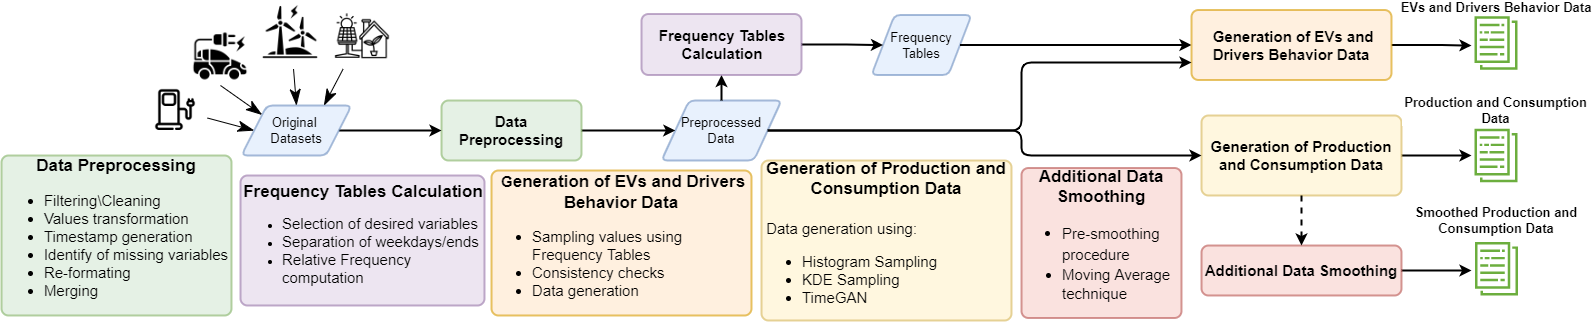
\includegraphics[width=0.81\linewidth]{Figures/ImplementationDiagram-ALL-paper.png}
  \caption{Schematic overview of workflow components in our system}
  \label{fig:dataflow}
  \Description{A Schematic overview of workflow components in our system. There are 5 basic components: Data Preprocessing, Frequency Tables Calculation, Generation of Driver Behavior Data, Generation of Production and Consumption Data and Additional Data Smoothing}
\end{figure*}

% We now provide an overview of our approach. 
The original collected data (from any available source) and the generated data is divided into two main categories: 
    {\em (a)} {\em energy production and consumption} and
    {\em (b)} {\em EVs' and drivers' behavior data}.
The first includes data related to the total consumption of renewable and non-renewable energy for a given region's infrastructure and the respective production. The second %ategory 
refers to EVs and their characteristics; %as well as 
the specifications of the available EV chargers; %Also, the input dataset consists of 
and to drivers' behavior, regarding the trips they perform, and the number of charging sessions and the time of the day these take place. %, as well as the trips they perform.
% However it is hard to generate consistent charging and trip events by sampling the frequency tables independently, since the most frequent values in both cases lie inside the same time intervals, i.e. an EV has high probability to be charging and en route at the same time, which is not realistic. To this end,
% %Since it is difficult to find consistent charging and trip events, 
% one has to enforce particular constraints for realism (as  detailed in  Section~\ref{subsec:driversdata}).

% Figure~\ref{fig:dataflow} shows the workflow and the components of our system. First, data is preprocessed to align values, generate compatible timestamps, and perform the required transformations and merging (see, Section~\ref{sec:prepro}). 
Figure~\ref{fig:dataflow} shows the workflow and the components of our system. First, data is preprocessed to generate compatible timestamps, consistent across all generated files, as the original data comes from different sources and has different formats. In addition, irrelevant and/or incomplete data is omitted, while some other is transformed to facilitate our work. We also extract new information---necessary for the data generation---by combining and merging data and files. 
% Section~\ref{sec:prepro} describes in detail the preprocessing step. 
In the case of energy production and consumption, the preprocessed dataset is fed directly to our proposed generation methods: histogram (HIST) and kernel density estimation (KDE) sampling~\cite{hardle2004nonparametric}, and time-series generative adversarial networks (TimeGAN)~\cite{zhang2018generative}. 
%and the results are obtained in the output.
For EVs' and drivers' behavior, computing the frequency tables of specific variables of interest (e.g., travel speed, time of connection, etc.) is also required. The calculated frequencies, along with specific constraint checks---in order to create realistic data and as close to the original---are used to generate the corresponding dataset. Finally, additional smoothing can be applied in the output.



\paragraph{User Configurations}
% \label{subsec:userConf}
%Our dataset generator is available for download via a github repository.
To generate data, the user can either {\em (a)} use a web-based GUI that eases the configuration of the generator, %(described in Sec.~\ref{sec:UI});
or {\em (b)} execute generation script templates and set
values to required configuration parameters via JSON files and the command line.
For the latter, %method, 
the user must specify: the number of EVs; the time horizon length; 
     the desired data generation technique among the available ones;
    the categories of EVs to be included in the generated dataset;
    the types of EV chargers to be considered; the additional smoothing parameters, if desired.
%the user must specify: 
%\begin{itemize}
 % \item the number of EVs
 %   \item the length of the time horizon
%    \item the desired data generation technique among the available ones
 %   \item the categories of EVs to be included in the generated dataset
  %  \item the types of EV chargers to be considered.
%\end{itemize}
% the number of EVs and the length of the time horizon; one of the alternative data generation techniques; specific categories of EVs to be generated; and potentially different types of chargers.
This information contains all required configurations for initiating the generation process.
% Then, the data generation process is initiated by executing the corresponding Python script.
The generated dataset comes in the form of CSV files, 
%which 
together with summarizing statistic tables and figures---specifically histograms, bar plots and time-series curves.
%, are provided in seperate folders.
Furthermore, any number of %new 
original datasets---different from the default 
%public one
included in our work---can also be incorporated for the training of the generation models. This is particularly helpful for organizations that need to protect private data, but are still in need to share anonymized information with third parties. 
The web-based GUI  uses a backend web server implemented in Flask---a Python micro web framework---while the frontend part was implemented using pure \emph{HTML} and \emph{JavaScript}. 
%The GUI contains a form with fields for every required configuration, either as drop-down lists or free text boxes. 

% runs locally and specifically on port 5004. In Appendix~\ref{appendixFigs} we provide screenshots of the GUI
%In what follows, we 
%We now give a detailed description of the input and output data, %as well as 
%and of the various constraints we impose to ensure the soundness of the %produced 
%results.

% \begin{figure}
%     \centering
%     %  \begin{subfigure}[b]{0.45\textwidth}
%     %      \centering
%          \includegraphics[width=0.45\textwidth]{Figures/UI_1.png}
%         %  \caption{}
%          \label{fig:UI1}
%     %  \end{subfigure}
%     %  \begin{subfigure}[b]{0.5\textwidth}
%     %      \centering
%     %      \includegraphics[width=\textwidth]{Figures/UI_2.png}
%     %      \caption{}
%     %      \label{fig:UI2}
%     %  \end{subfigure}
%     \caption{Screenshot of the web-based user interface}
%     \label{fig:UI}
%     \Description{Screenshot that shows the GUI of our system.}
% \end{figure}
\section{Results Overview}


%%%%%%%%%%%%%%%%%%%%%%%%%%%%%%%%%%%%%%%%%%%%%%%%%%%%%%%%%%%%%%%%%%%%%%%%%%%%%%%%%%%%%%
% \section{Data Acquisition and Preprocessing}
% \label{sec:prepro}

% % Most of the data related to EVs and Smart Grid are collected by utilitiy or multinational companies. However, these companies have a legal obligation not to share them publicly. Nevertheless, as we have already mentioned, the availability of such data is necessary for further research in the domain. There are several ways that in combination with the tool we present, could make realistic data available to the public.

% % For example, companies could anonymize a small portion of their customers, perhaps a few hundred, to make anonymous data publicly available and then anybody could use the data generator to produce data for thousands of customers. Additionally, in case that the company does not want to publish real data, even if it is anonymous, it could publish a representative sample of them. For example, a company holds data for thousands of consumers. It could apply them a K-means algorithm~\cite{likas2003global} in order to group them into clusters and then give the researcher the centers of the clusters rather than the actual measurements. In addition the researcher could work in a way similar to ours. That is, to collect various data from different sources and then combine it through the data generator in order to produce new data.

% This section describes our datasets, and the functionality of the `Data PreProcessing' module. 
% % where all data is pre-processed.
% The original data comes from different sources and has different formats. 
% Therefore, we need to apply specific transformations, and then combine it properly in order to end up with the final input files.
% Therefore, appropriate transformations must be performed to come up with an acceptable format.
% Table~\ref{tab:dataInfo} provides an overview of the form of input and output data. % of our system.


% \begin{table*}[h]
%     \caption{Description of input and output data}
%     \label{tab:dataInfo}
%     \begin{tabular}{cll}\toprule
%     \textit{Data Category} & \multicolumn{1}{c}{\textit{Input of `Data Preprocessing' Component}} & \multicolumn{1}{c}{\textit{Output of Dataset Generator}}\\ \midrule
%     \begin{tabular}[c]{@{}c@{}}Production\\ and\\  Consumption\\ Data\end{tabular} & \begin{tabular}[c]{@{}l@{}}\textbf{Production}: DayTimeOfMeasurement (start-end), \\ Lignite, FossilGas, Solar, Wind\\ \textbf{Consumption}: DayTimeOfMeasurement (start-end), ActualTotalLoad\\ \textbf{*}irrelevant or/and incomplete elements are omitted (e.g. Area, FossilOil etc.)\end{tabular} & \begin{tabular}[c]{@{}l@{}}Date, Year, MonthOfYear,\\ DayOfWeek, TimeOfDay, LigniteGen,\\ FossilGasGen, SolarGen,WindGen,\\ TotalLoad, ImportExport\end{tabular}\\ \midrule
%     \begin{tabular}[c]{@{}c@{}}EVs \\ and \\ Drivers \\ Behavior \\ Data\end{tabular} & \begin{tabular}[c]{@{}l@{}}\textbf{EVs specs}: CarModel, BatteryCapacity, MaximumDCChargingPower,\\ MeanEnergyConsumption,Category \\ \textbf{Chargers specs}: ChargerType, ChargerRating, ACDC, RatedPower\\ \textbf{Drivers Behavior-Charging events}: ParticipantID\\ BatteryChargeStartDate, BatteryChargeStopDate,\\ StartingSoC, EndingSoC\\ \textbf{Drivers Behavior-Trip events}: ParticipantID, TripStartDateTime,\\ TripStopDateTime, TripDistance, PowerConsumption\\ \textbf{*}irrelevant elements are omitted (e.g. Length, Wheelbase etc.)\end{tabular} & \begin{tabular}[c]{@{}l@{}}Date, DriverID, Year, MonthOfYear,\\ DayOfWeek, TimeOfDay, EVModel,\\ BatteryCapacity, Category,\\ MeanEnergyConsumption,\\ MaxDCPower, Status, StartingSoC,\\ EndingSoC, ChargerType,\\ ChargerPower, ChargingTime,\\ ChargingConsumption, \\ TripTime, TripDistance,\\ TripConsumption\end{tabular}\\ \bottomrule
%     \end{tabular}
% \end{table*}


% \begin{table*}[]
%     \caption{Datasets used}
%     \label{tab:datasetsTable}
%     \begin{tabular}{ccc} \toprule
%     \textbf{Company/Platform} & \textbf{Dataset Description} & \textbf{Preprocessed Data} \\ \midrule
%     \begin{tabular}[c]{@{}c@{}}My Electric Avenue\\ {\scriptsize\url{https://eatechnology.com/resources/projects/my-electric-avenue/}}\end{tabular} & \begin{tabular}[c]{@{}c@{}}EV driving behavior and charging\\  data from up to 200 EVs\end{tabular} & \begin{tabular}[c]{@{}c@{}}1 CSV file for Charging Events \\ 1 CSV file for Trip Events\end{tabular} \\ \hline
%     \begin{tabular}[c]{@{}c@{}}ENTSOE transparency platform\\ {\scriptsize\url{https://transparency.entsoe.eu/dashboard/show}}\end{tabular} & \begin{tabular}[c]{@{}c@{}}Measurements concerning the Actual\\ Generation per Production Type and the Actual\\ Total Load for all European regions\end{tabular} & \begin{tabular}[c]{@{}c@{}}1 CSV file for Production \\ \& Consumption Data\end{tabular} \\ \hline
%     \begin{tabular}[c]{@{}c@{}}Mendeley Data platform\\ {\scriptsize\url{https://data.mendeley.com/datasets/tb9yrptydn/2}}\end{tabular} & \begin{tabular}[c]{@{}c@{}}Electric passenger cars\\ with theirspecifications\end{tabular} & \multirow{2}{*}{\begin{tabular}[c]{@{}c@{}}1 CSV file for \\ EV characteristics\end{tabular}} \\ \cline{1-2}
%     \begin{tabular}[c]{@{}c@{}}Tesla\\ {\scriptsize\url{https://www.tesla.com/en\_EU/support/european-union-energy-label}}\end{tabular} & Technical features of Tesla models &  \\ \hline
%     \begin{tabular}[c]{@{}c@{}}Spirit Energy\\ {\scriptsize\url{https://www.spiritenergy.co.uk/kb-ev-understanding-electric-car-charging}}\end{tabular} & Specifications of EV's chargers & \begin{tabular}[c]{@{}c@{}}1 CSV file for EV \\ chargers specifications\end{tabular}\\
%     \bottomrule
%     \end{tabular}
% \end{table*}

% \subsection{Energy Production and Consumption Data}
% \label{subsec:energydata}

% %In this category,
% % we have time-series data following 
% This data comes in time-series format, following
% the structure of the ENTSOE transparency platform. %\footnote{\url{https://transparency.entsoe.eu/dashboard/show}} 
% This includes real measurements (available online, free of charge) concerning the aggregate generation levels per production type, as well as aggregate demand for all European regions for the recent years. 
% %This information is available online, free of charge.
% Our main input consists of CSV files, having $n \in \mathbb{N}$ rows and $c \in \mathbb{N}$ columns. 
% Each row corresponds to a series of measurements for a configurable time interval (e.g., an hour of the day), while each column contains information about ({\em a}) the particular date and time, ({\em b}) the measurements of the actual generation per production type (e.g., Fossil Gas, Solar, Wind), and ({\em c}) the total load consumption. All measurements are in {\em kWh}. The output file has a similar format (see Table~\ref{tab:dataInfo}).
% % {\color{red}For example, given hourly measurements and a time horizon of 30 days, the number of rows would be $30\cdot 24=720$, while the columns correspond to the particular date (i.e., year, month, day of week, time of day) and the different production/consumption measurements from each type.}


% \subsection{EVs and Drivers Behavior Data}
% \label{subsec:driversdata}
% As we can see in Table~\ref{tab:datasetsTable} the data related to electric vehicles comes from many different sources and the main difference to the previous case is that in this category there is no time-series format. For the characteristics of EVs, the input dataset comes mainly from the online, publicly available Mendeley Data platform, %\footnote{`Dataset of electric passenger cars with their specifications', \url{https://data.mendeley.com/datasets/tb9yrptydn/2}.} 
% while this data can easily be augmented with additional information from other sources. For example, we also add some technical features of Tesla models %available from the official website of Tesla in Europe, %\footnote{\url{https://www.tesla.com/en_EU/support/european-union-energy-label}} 
% which were not included in the initial Mendeley dataset.
% The combination of these two data sources
% %is used to construct a second CSV file 
% provides information regarding EV technical characteristics, such as the equipped battery specification and the overall energy consumption of the EV.
% %Here, the number of rows corresponds to different EV models, and the number of columns to the various characteristics
% Information about the different types of the available chargers (AC or DC, Regular socket, Single phase, or 3 phases), their charging speed and their rated power is based on the``Spirit Energy'' website.
% % A different input CSV file, produced during preprocessing, is used to dictate the specifications of the available chargers, based on the``Spirit Energy'' website, %\footnote{\url{https://www.spiritenergy.co.uk/kb-ev-understanding-electric-car-charging}} 
% % and it contains the different types of chargers (AC or DC, Regular socket, Single phase, or 3 phases), their charging speed and their rated power.

% Finally, the data related to the drivers' driving behavior comes from the `My Electric Avenue' project. %\footnote{\url{https://eatechnology.com/resources/projects/my-electric-avenue/}} 
% There,  participants monitored the usage of over 200 EVs, a number of low voltage networks, and the switching of the EVs to support those networks. The trial participants’ charging and driving behavior was recorded using the EVs’ telematics systems. We utilize two files from that project: the first one contains information about the times each EV charged, as well as the state of charge for each time an EV is connected and charged; and the second one, contains distance, times, and power consumption information for each of the recorded drivers' trips.

% \subsection{Data Preprocessing}
% \label{subsec:datapre}

% As already mentioned, the original data has different formats, therefore, we need to apply specific transformations, and then combine it properly in order to end up with the final input files. As a first step of the generation process, we preprocess the acquired data files to assign them appropriate timestamps. That is, we transform their day and time information  to a timestamp %that is 
% consistent across all generated files, i.e., \emph{Date, Year, MonthOfYear, DayOfWeek, TimeOfDay}).

% Next, regarding EV characteristics, the data from the Mendeley platform is considered in its original format, and missing information about the technical features of some EV models is filled in by taking into account other online sources. In addition, a new column `Category' is inserted that signifies different EV types according to battery capacity. All aforementioned data is combined into a single file, apart from the information of the EV chargers which is provided in a seperate one (see Table~\ref{tab:datasetsTable}). 

% As for charging events-related data, the corresponding file (see Table~\ref{tab:datasetsTable}) contains the exact dates and times that charging events start and end, as well as the EV battery state of charge at the beginning and at the end of a charging event, noted as \emph{StartingSoC} and \emph{EndingSoC}, respectively. Again, we assign compatible timestamps to each event and normalize the state of charge values to the $[0,1]$ range. %interval.
% Each row 
% %of the file
% represents a charging event/action, and each column includes data related to the charging events, i.e. the exact time of charging events, duration of charges, and the status of the battery. Finally, two additional columns are inserted: \emph{SoCDiff}, which contains the difference `\emph{EndingSoC}- \emph{StartingSoC}', indicating the percentage of the battery that was charged during a charging event; and \emph{ChargingTime}, expressing the duration (in minutes) of each charging event, as calculated from its {\em start} and {\em end} timestamps.

% Regarding the data related to the trip events, the file (see Table~\ref{tab:datasetsTable}) has the same format as that of the charging events: each row represents a trip event/action and each column, the exact time of a trip event, the duration of the trip, the trip distance and the power consumed during each trip respectively. By extension, we followed similar techniques in order to pre-process the data. We converted the start and end dates of the trip events into the appropriate format and used them to calculate the duration of each event (in minutes), in a new column called \emph{TripTime}. Lastly, we calculate the velocity of the vehicles through a simple time-distance relationship, assuming that the vehicle performs linear motion with constant speed.

% In terms of the generated synthetic data output files (\emph{EVs and Drivers Behavior Data} in Figure~\ref{fig:dataflow} and Table~\ref{tab:dataInfo}), their number is proportional to the number of drivers that the user has specified. %as a configuration. 
% For each one, the number of rows corresponds to measurements for a particular time interval, and each column represents the characteristics of each driver's EV, detailed information about charging events 
% %(i.e., exact time of charging event, duration of charge and status of the battery)
% and the characteristics of the charger with which a charging event takes place.
% %(i.e., AC or DC, single-phase or 3-phase, charger’s charging speed and rated power)
% Finally, detailed information on trip events are provided.
% %(i.e., exact time of a trip event, the duration of a trip, the distance travelled and the power consumed during each trip).
% In addition, since the columns of the output files refer to both charging and trip events, in case of a charging event the columns related to the trip event are empty and vice versa. If neither event takes place, all  aforementioned columns are left empty.

% The other data category, energy production and total consumption, originates from the ENTSOE platform and comes in the form of 8 CSV files, 4 for actual generation and 4 for total load, one for each year, from 2017 to 2020. The preprocessing is performed on a yearly basis. First, we convert the timestamp to the appropriate format and then we combine the production and consumption data into a common file (see Table~\ref{tab:datasetsTable}) %and remove all incomplete rows (if any). 
% We then insert a new column that holds the imbalance between the aggregates of consumption and production. A resulting positive number indicates that energy is imported from neighbouring regions; otherwise, it is exported.
% %%%%%%%%%%%%%%%%%%%%%%%%%%%%%%%%%%%%
% \section{Data Generation Techniques}
% \label{sec:gen}

% In this section, we present our dataset generation process, which uses different statistical methods to produce synthetic data.
% There are two desired types of data to generate: 1) energy consumption and production, 2) EVs and drivers behavior data. For the former, we adopt three different generation methods that can be used interchangeably:
% {\em Histogram Sampling}; 
% {\em KDE Sampling}; and {\em TimeGAN}.
% Since the drivers' 
% %driving 
% behavior data %, which 
% do not come in a time series format, the application of these methods is not meaningful. Therefore, we also put forward a {\em Frequency Tables Method}, which requires no such assumption for the input. Algorithm~\ref{algo1} gives the general picture of the operation of our system, while algorithms~\ref{algo2} and~\ref{algo3} describe the dataset generation process for the production and consumption data and the drivers' behavior data respectively.

% \begin{center}
% % \scalebox{0.95}{
% % \begin{minipage}{0.9\linewidth}
% \begin{algorithm}[h]
% \caption{Dataset Generation}
% \label{algo1}
% \begin{algorithmic}[1]
%     \State Read the input $json$ file with user's options
%     \State Create the output folder \Comment{All generated files stored here.}
%     \State Generate Energy Production \& Consumption Data, Algorithm~\ref{algo2}
%     \State Generate Drivers' Behavior Data, Algorithm~\ref{algo3}
% \end{algorithmic}
% \end{algorithm}
% % \end{minipage}
% % }
% \end{center}

% \subsection{Histogram Sampling}
% \label{subsec:histsampl}
% In the Histogram Sampling case, we create a dataframe with size respective to the time period given by the user, and then fill in all the columns related to the date and time variables.
% % Next, we define the measurements of the original data that we need to consider for each column/variable. 
% % By analyzing and plotting the time-series of each variable for intervals of one week, we sought to find peaks, periodicity and irregularities within this time period. Therefore after visual inspection, we recorded how variables are related to the month, day and time, and so we group each column based on the observed time dependence. For the total load consumption we take into account the month, day and hour; while for Solar and FossilGas generation we keep the month and time of day; and finally, for the Lignite and Wind generation, for which no pattern was observed for the day and time, we take into account only the corresponding month of the year.

% Subsequently, for each variable,
% % having a series of measurements in each group, 
% we create a histogram with a default number of bins.
% In general, we could construct a histogram with an arbitrary number; the more the bins, the more precise the sampling will be, but at the same time, most of the bins should contain a sufficient number of counts to be statistically significant. By conducting exploratory experiments, 
% %in the search for the optimal number of bins, we concluded 
% %that the best value is the one for which the bins have an average population of at least 5 elements.
% we converged to an empirically ``optimal'' number of bins such that they have an average population of at least 5 elements.

% To generate values using a histogram, we first calculate the corresponding cumulative distribution, and then sample a random number from a uniform distribution between 0 and 1. 
% This random sample indicates a point in the x-axis of the CDF, from which we find the respective y-axis value, which constitutes our final synthetic dataset value.
% In this way, for each row of data we sample a new value for the selected column. The process is repeated for every column of the preprocessed file (see Table~\ref{tab:datasetsTable}).

% In cases where the values that we sample refer to \emph{SolarGen}, we perform an additional check as values are expected to be equal to zero during night time and low during cloudy days. 
% %Due to the physical environment model (day and night), we expect measurements to be equal to zero during night hours, or to be smaller during cloudy days.
% However, mainly due to faulty measurements, there are rare cases where the original values are quite close to zero, but different than zero, thus forming non-zero probability mass for a positive value to come up, even during night hours. Thus, to avoid large inconsistencies with non-zero values during hours when it is not plausible (e.g., during night hours), in cases where the sample has a value less than a minimum level (as this is inferred by the original datasets), we treat it as zero. As we saw in practice, this intervention helps towards a better fit between the real data in the input and the generated data in the output, as shown in our experimental results in Section~\ref{sec:results}.

% \begin{center}
% % \scalebox{0.95}{
% % \begin{minipage}{0.9\linewidth}
% \begin{algorithm}[h]
% \caption{Generate Production \& Consumption Data}
% \label{algo2}
% \begin{algorithmic}[1]
%     \State Create dataframe $df$ according user's time horizon
%     \If{$method = HIST$} \Comment{The method is chosen by the user.}
%         \State Apply HIST method \Comment{Histogram Sampling, see Section~\ref{subsec:histsampl}}
%     \ElsIf{$method = KDE$}
%         \State Apply KDE method \Comment{KDE Sampling, see Section~\ref{subsec:kdesampl}}
%     \ElsIf{$method = TimeGAN$}
%         \State Apply TimeGAN method \Comment{TimeGAN, see Section~\ref{subsec:timegan}}
%     \EndIf
%     \State Save $df$ to $.csv$ file    
%     \If{$Additional Smoothing = True$} \Comment{User set parameter.}
%         \State Take the smoothing parameters (rolling window) for each variable \Comment{Histogram Sampling, see Section~\ref{subsec:histsampl}}
%         \State Apply smoothing on $df$ and save smoothed data to new $.csv$ file\Comment{Data Smoothing, see Section~\ref{subsec:smoothing}}
%         \State Create figures and metrics for Smoothed Generated Data
%     \EndIf
%     \State Create figures and metrics for Generated Data
% \end{algorithmic}
% \end{algorithm}
% % \end{minipage}
% % }
% \end{center}
% \begin{center}
% % \scalebox{0.95}{
% % \begin{minipage}{0.9\linewidth}
% \begin{algorithm}[h]
% \caption{Generate Drivers' Behavior Data}
% \label{algo3}
% \begin{algorithmic}[1]
%     \For{each EV}\Comment{Number of EVs is chosen by the user}
%         \State Create dataframe $df$ according user's time horizon
%         \State Fill in the columns of $df$ related to date and time
%         \State Create an empty dataframe $df\_s$ \Comment{To store variables that will be sampled only once (DriverID \& EV specs)}
%         \State Calculate $numOfDays$ \Comment{The number of days corresponds to user's time horizon}
%         \State Sample the num of daily charges for every $numOfDays$
%         \State Create Sample Storage for weekdays, Algorithm~\ref{algo4} $Sampling\_Charge\_Data(0,numOfDays*4,0,df\_s,0,2,0)$
%         \State Store DriverID \& EV specs to $df\_s$
%         \State Create Sample Storage for weekends: Algorithm~\ref{algo4} $Sampling\_Charge\_Data(0,numOfDays*4,0,df\_s,0,2,1)$
        
%         \If{$checksMode = Strict$} \Comment{choosing a checksMode}
%             \State $StrictConstraintsDataGeneration()$, Alg.~\ref{algo5}\Comment{See Section~\ref{subsec:dribehgen}}
%         \ElsIf{$checksMode = Looser$}
%             \State Apply Looser Constraints mode\Comment{See Section~\ref{subsec:dribehgen}}
%         \ElsIf{$checksMode = Min$}
%             \State Apply Absolutely Necessary Constraints mode\Comment{See Section~\ref{subsec:dribehgen}}
%         \EndIf
    
%         \For{the whole $df$}
%             \State Find 2 consecutive charges
%             \If{$Starting\_SoC of 2nd < Ending\_SoC of 1st$}
%                 \State $CreateTripEvent()$, Algorithm~\ref{algo6}
%             \EndIf
%         \EndFor
%         \State Save $df$ to $.csv$ file
%     \EndFor
%     \State Merge all $.csv$ files to 1 file
%     \State Create figures and metrics for Generated Data
% \end{algorithmic}
% \end{algorithm}
% % \end{minipage}
% % }
% \end{center}
% \subsection{KDE Sampling}
% \label{subsec:kdesampl}

% In this case we calculate the kernel density estimates of the original production and consumption data over the entire time horizon.
% %{\color{red}, using Python's machine learning library scikit-learn.}

% Kernel density estimation (KDE) is a non-parametric method for estimating the probability density function of a given random variable. Given a sample of $n$ independent, identically distributed (i.i.d) observations ($x_1,x_2,…,x_n$) of a random variable from an unknown distribution at any given point $x$, the kernel density estimate is given by:
% \begin{eqnarray}
% p(x) & = & \frac{1}{nh} \sum_{j = 1}^{n}K\left(\frac{x-x_j}{h}\right)
% \end{eqnarray}

% \noindent
% where $K(x;h)$ is the kernel function and $h$ is the smoothing parameter, also called the bandwidth. There is a wide range of kernel functions, such as Gaussian, Top Hat, Exponential, Linear, Cosine, Epanechnikov and others. In our approach we use the Gaussian kernel,
% %$K(x;h) \propto exp(-\frac{x^2}{2h^2})$, 
% since it is one of the most widely used kernel functions and is shown to perform well. Having set a specific range in bandwidth, we tune the bandwidth parameter via cross-validation and select the parameter value that maximizes the log-likelihood of data. Therefore, similarly to Histogram Sampling, after selecting the corresponding subset of data ($x_1,x_2,…x_n$), where $n$ is the the subset's length), we sample a new value for the selected column and the process is repeated for all columns. 
% Also, as described earlier, in the case of \emph{SolarGen} we perform the corresponding checks.


% \subsection{Time-series GANs}
% \label{subsec:timegan}

% {\em Time-series Generative Adversarial Networks (TimeGANs)}~\cite{yoon2019time} are 
% %GAN based models, 
% able to generate time-series data that preserve temporal dynamics, in the sense that new sequences respect the original relationships between variables across time. Unlike other GAN architectures where unsupervised adversarial loss on both real and synthetic data is implemented, TimeGAN introduces the concept of supervised loss: the model is encouraged to capture time-dependent %conditional 
% distribution within the data by using the original data for supervision; and synthesizes sequential data composed by four networks with distinct roles in the data modelling process: the generator, the discriminator, and recovery and embeddings models.\footnote{To implement TimeGAN we used part of the code publicly available in the github repository ydata-synthetic, which develops various GANs using Tensorflow 2.0~\cite{ydata}.}

% Three types of losses are considered, the {\em reconstruction}, {\em supervised}, and {\em  unsupervised} loss.
% The first  refers to embeddings and the comparison between the original and reconstructed (generated) data; the second and third to the approximation of the time dimension in the latent space, and the relationship between the generator and the discriminator, respectively.

% Given the network architecture and the losses defined above, there are 3 training phases:
% First, we train the autoencoder on the provided sequential data to optimally reconstruct it; then, the supervisor is trained using real data sequencies to capture the historic temporal relationships; and finally, the combined training of the four networks, while minimizing all three loss functions.

% Note that, in the case of TimeGAN, the time dimension of the input data matches that of the output.
% Thus, in this case, the input data must be further pre-processed, first to normalize values, then to create rolling windows across the temporal dimension, and  finally to shuffle observations in order for them to meet the i.i.d. property. 
% Furthermore,
% %due to the structure of the model, the generated data has the same size as the input. % data. 
% %Therefore, 
% since the ENTSOE-provided input data is for 1 or 4 years, this method can be used to generate 1 or 4 years of synthetic data respectively. However, input data with a different time horizon can be used, as long as it 
% respects the format specified in Section~\ref{subsec:energydata}.
% %has the same format as ours.




% \subsection{Frequency Tables Method}
% \label{subsec:dribehgen}

% We now discuss the Frequency Tables method, used to generate the drivers' behavior data.
% Here, the data is generated based on frequency tables and files including information regarding the EV characteristics.
% The Frequency tables are used to determine the probability of an event happening at a particular time instant, by counting the original dataset values.
% To construct them, we read the files related to the charging and trip events, and create 2 for each of the following 5 variables:

% \begin{itemize}
%     \item Charge Start Hour: The hour that a charging event begins
%     \item Daily Charges: The number of daily charges an EV makes
%     \item Starting SoC: The EV's SoC when a charging event begins
%     \item Ending SoC: The SoC when a charging event ends
%     \item Trip Velocity: The average speed of the EV during a trip
% \end{itemize}

% More specifically, the two files we create for each of the above variables (see \emph{Frequency Tables} in Figure~\ref{fig:dataflow}) correspond to a relative frequency table for weekdays and another one for weekends. A relative frequency table shows the `popularity' of a particular value, based on the input data. In order to find the relative frequency of each value, we count how often a data value (or values' range) appears in the original data, and then scale it by dividing it with the total number of counts across all values. 
% The relative frequency indicates the number of times a specific (range of) value(s) has been observed, compared to the total number of measurements. Thus, each of the relative frequencies correspond to the weight of a specific value, which we use later during the sampling process. The larger the weight, the greater the probability the specific value will appear in the output.

% We now 
% %proceed to 
% describe the main process for this part of our system. As outlined in Alg.~\ref{algo3}, it is repeated for each EV, until the number of EVs/drivers chosen by the user is completed.
% % To generate EVs and driver behavior data, we repeat the following process for a number of times, equal to the user specified number of EVs that the dataset needs to have.
% % First, we create a dataframe according to the time period given by the user and then we fill in all the columns related to the date and time variables, just as described earlier.
% % Then we calculate the number of days that correspond to the time period entered by the user and for each one of them, we sample the number of daily charges from the corresponding frequency table.
% % Then we sample charging events from the respective frequency table, and fill in the cells of the dataframe. We must also point out that some data (DriverID and the specs of the EV) is sampled only once for each driver and remains unchanged throughout the file.
% Each time a new charging event is sampled, we check if the corresponding starting time is later than the end of the previous charging event's end. Also, the \emph{StartingSoC} should be smaller than the \emph{EndingSoC} of the preceding event's. However,  to avoid constant data sampling from various Frequency Tables, every time we need data related to charging events, we create a storage of samples (Alg.~\ref{algo4}, in Appendix~\ref{algo}).
% % Through a method (\emph{Sampling\_Charge\_Data()}) we sample the maximum number of charging data that correspond to the number of days we calculated earlier (i.e.
% % \begin{math}
% %   sampling\_data (n) = charging\_data\_for\_1\_charge \times 4charges\_a\_day \times Ddays
% % \end{math}
% % ).
% % Algorithm~\ref{algo4}, in the Appendix~\ref{algo}, shows how \emph{Sampling\_Charge\_Data()} works in case of the initial creation of the aforementioned storage of samples. 
% % Therefore, if the conditions are met, we randomly pick a sample from the storage, otherwise we try to pick a new sample that meets our requirements. If there is no such sample,
% % % we call the \emph{Sampling\_Charge\_Data()} method but with different arguments. 
% % % The method works as in the previous case with the difference that it returns only 1 
% % we create a new charging sample that meets our requirements.


% \begin{table*}[h]
%     \caption{K–S statistic of Production and Consumption Data. Best performance results indicated in bold.}
%     \label{tab:metricsLoad}
%     \begin{tabular}{c|c|ccccc|c}\toprule
%     \textit{Output Data time-horizon} & \textit{Method} & \textit{LigniteGen} & \textit{FossilGasGen} & \textit{SolarGen} & \textit{WindGen} & \textit{TotalLoad} & \textit{Average} \\ \midrule
%     \multirow{3}{*}{4 years of data} & HIST & 0.005 & 0.005 & \textbf{0.03} & \textbf{0.004} & 0.005 & \textbf{0.01} \\
%      & KDE & \textbf{0.004} & \textbf{0.004} & 0.036 & \textbf{0.004} & \textbf{0.004} & \textbf{0.01} \\
%      & TimeGAN & 0.08 & 0.038 & 0.459 & 0.06 & 0.035 & 0.134 \\ \midrule
%     \multirow{3}{*}{1 year of data} & HIST & 0.011 & 0.011 & \textbf{0.031} & \textbf{0.009} & 0.009 & \textbf{0.014} \\
%      & KDE &\textbf{0.001} & \textbf{0.006} & 0.038 & 0.01 & \textbf{0.007} & \textbf{0.014} \\
%      & TimeGAN & 0.052 & 0.072 & 0.464 & 0.068 & 0.044 & 0.14 \\ \bottomrule
%     \end{tabular}
% \end{table*}

% \begin{table*}[h]
%     \caption{Difference of Drivers Behavior Data Frequency Tables}
%     \label{tab:metricsEV}
%     \begin{tabular}{c|cccccc|c}\toprule
%     \textit{Method} & \textit{DailyCharges} & \textit{ChargeStartHour} & \textit{StartingSoC} & \textit{EndingSoC} & \textit{DailyTrips} & \textit{TripStartHour} & \textit{Average} \\ \midrule
%     \textbf{StrictChecks} & 0.419 & \textbf{0.057} & 0.079 & 0.231 & 0.821 & \textbf{0.345} & 0.325 \\
%     \textbf{LooserChecks} & 0.095 & 0.232 & 0.077 & 0.227 & 0.619 & 0.465 & 0.286 \\
%     \textbf{MinChecks} & \textbf{0.072} & 0.173 & \textbf{0.067} & \textbf{0.221} & \textbf{0.057} & 0.453 & \textbf{0.26} \\ \bottomrule
%     \end{tabular}
% \end{table*}

% With the respective configuration parameter, the user can choose among the different dataset generation algorithms.
% % the algorithm to be executed for the dataset generation processe varies depending on the user's choice. %Therefore we have 3 options available:
% Now, since the generation process is based on random sampling, it is probable that the output might not adhere to real-world constraints in some cases, e.g. an EV discharging more that it would be possible between charging events, or a charge event appearing before the previous being completed.
% For this reason, to better control the level of constraints that will be enforced throughout the generation process, we provide three different modes:
% {\em Strict constraints} where the time intervals that the EVs charge are finely dispersed throughout the day, 
%     {\em Looser constraints} where charges must be completed within the same day, and
% {\em Absolutely necessary constraints}, i.e. there are no time restrictions regarding when an EV begins charging.


% In all these modes, the focus is %put on 
% on the number of daily charges.
% The description of the {\em Strict constraints} mode is shown in Algorithm~\ref{algo5}, in Appendix~\ref{algo}. 
% In case only one charging event is sampled, then no special action is required.
% % Initially, if the number of daily charges is equal to 1 then we fill in the dataframe, according to the sample we have chosen.
% If the number of daily charges is 2, then we divide the day into two 12-hours and carry out the 1st charge. If the end of the charge is within the first 12-hours, then we take a new sample and carry out the 2nd charge. In case the number of charges is equal to 3, we first divide the day into three 8-hour periods, and carry out the 1st charge. If the end of the charge is within the first 8-hour period, %then 
% we take a new sample and perform the 2nd charge. Similarly, we check if the end of the current charge is within the second period and we perform the 3rd charge. However, in case the 1st charge is not completed within the first period, we check if it is completed within the second, so that then at least the 2nd charge can be performed. The same rationale applies %also %case of 
% for 4 or more daily charges, where we perform similar steps.

% For the looser constraints, the only check that is performed before sampling the next charging event, is that the previous charge should have been completed before 23:00 of the same day. Finally in the absolutely necessary constraints, there is no extra rule, apart from that the \emph{StartingSoC} 
% during a charging event must be lower than the \emph{EndingSoC} 
% of the preceding one. 
% In all 3 modes we sample different frequency tables for weekdays and different for weekends.
% %, respectively.
% % by using the corresponding Frequency tables as input.

% After filling the basic dataframe with the charging events, it is then rescanned in order to fill in the necessary trip events between the successive charging events (see Algorithm~\ref{algo6} in Appendix~\ref{algo}). The rationale behind this part is that if there is power consumption between two consecutive charges, a trip event %should 
% must have intervened.
% %been mediated. 
% The only variable that is sampled and is related to a trip event, is the velocity of the EV. The trip information is thus filled in by sampling the velocity and by %also 
% calculating the remaining parameters related to EVs  (i.e., \emph{TripTime}, \emph{TripConsumption} and \emph{EndingSoC}).

% % Regarding the EV velocity values during the trips, they are grouped by 5 units, and are calculated based on the time and distances of the trips in the original input data. Now, in case the time interval between 2 consecutive charges is not enough to accomplish a trip event with some of the available velocity values, then the minimum speed required for the trip completion is calculated and is assigned as the EV’s velocity in that trip. Therefore, in some cases the velocity of a trip event might exceed 100 km/h, which is the maximum velocity of a car in the original dataset.


% \subsection{Data Smoothing \& Curve Matching}
% \label{subsec:smoothing}
% Due to the fact that our samples are independent, it is possible that consequtive time-points are not as smooth as the real time-series for the cases of Production and Consumption data. To overcome this we provide data smoothing techniques that the user may apply to the generated output.
% % Regarding the Production and Consumption Data, the user has the ability to apply additional smoothing on them. 
% The smoothing method that we use is the moving average technique.

% The moving average, also known as rolling mean, is commonly used upon time series to smooth random short-term variations and to highlight other components that are present in the data, such as trends, season, or cycle. 
% %There are many types of moving averages, such as, the simple moving average (SMA), the cumulative moving average (CMA), and the exponential moving average (EMA). 
% In our case we use the simple moving average (SMA), which is the unweighted mean of $m$ data points. The selection of $m$,  the {\em sliding} or {\em rolling window}, depends on the degree of smoothing the user desires, since increasing the value of $m$ results to more smooth curves, but at the expense of accuracy. Thus the window size is specified by the user, as described in Section~\ref{sec:methodOver}.
% % {\color{red} as seen in Fig.~\ref{fig:UI}(b).} 
% %For a sequence of values, we calculate t
% The simple moving average at time period t is:
% %as follows:
% \begin{eqnarray}
%   SMA_t = \frac{x_t+x_{t-1}+x_{t-2}+...+x_{m-(t-1)}}{m}
% \end{eqnarray}

% \noindent
% where $x$ is the variable (e.g., SolarGen in our dataset) and $t$ is the current time period (e.g. the time horizon of our dataset).
% %We calculate the simple moving average by using the ``pandas.Series.rolling'' method. This method provides rolling windows over the data. On the resulting windows, we can perform calculations using a statistical function (in this case the mean).


% In addition, to produce data even closer to the originals, we perform a pre-smoothing procedure. First we check the CSV file of the generated data (\emph{Production and Consumption Data} in Figure~\ref{fig:dataflow} and Table~\ref{tab:dataInfo}). For each value of a specific variable (e.g. SolarGen) we calculate the mean of the values for a time horizon of 24 hours, 12 hours before and 11 hours after the specific time interval. Then we randomly select a value from the original data set, which corresponds to the month, day and time we are in, and we calculate in the same way the corresponding mean. Afterwards, we compare the two means, having already calculated their difference. If the mean of the original data is greater than that of the generated ones, we add the difference to the value we have; otherwise we subtract it. The  process is applied to the entire file, for each variable. %Thus, by applying these two techniques the time series curves of the generated data fit better those of the original.

% % \section{Web-Based User Interface}
% % \label{sec:UI}

% % The previous sections presented in detail the functions of our system, as well as the techniques are used to produce synthetic data. In addition to the basic functions described, we have created a web-based user interface (UI), which helps the user to easily handle our Dataset Generator. The UI uses a backend web server, implemented in Flask\footnote{https://flask.palletsprojects.com/en/2.0.x/}--a Python micro web framework-- while the frontend part was implemented using mainly \emph{HTML} and \emph{JavaScript}. 
% % The UI runs locally and specifically on port 5004.
% % %So the user firstly runs the \emph{Flask\_App.py} file and then opens a new tab of a web browser, at `localhost: 5004'.
% % %This is the URL of the UI, which can be used to perform all the procedures described in section~\ref{sec:gen}.

% % % The UI\footnote{Web UI screenshots are provided in the Appendix.} allows the user to first select the time horizon for the data set (start and end date) and one of the 3 available techniques for the generation of Production and Consumption Data. She  then enters the number of EVs, as well as the percentages of the EV categories (A, B and C), which correspond to the number of EVs--from each category--that will be in the dataset. Afterwards, the user, for each category of EV chargers (Slow, Fast and Rapid) sets the probability of selecting a charger of a specific category, during the generation of the dataset. In a fairly large data set, these probabilities also reflect the percentages of each category on the total amount of the chargers. Subsequently, the user can apply additional smoothing to the generated Production and Consumption Data, by setting the rolling window for each variable. 
% % % %Subsequently the user enters the name of the folder from which he wants the input data to be retrieved. The default name is `InputData', and it contains our original data.
% % % Finally, the user selects the `Generate Data' button and once all the necessary values have been filled in correctly, the generation of the synthetic data and the corresponding figures and statistics begins.

% % In addition to the above, the user can generate figures and statistics for data he has already generated. On the second tab of the UI, the user can select folders for the original and generated data, and by pressing the corresponding submit button, the figures and statistics of the corresponding data are automatically created.
% % }

% %%%%%%%%%%%%%%%%%%%%%%%%%%%%%%%%%%%%%%%%%%%%%%%%%%%%%%%%%%%%%%%%%%%%%%%%%%%%%%%%%%%%%%
% \section{Experimental Evaluation}
% \label{sec:results}
We compare the distributions of the original data considered as input, to those of the synthetic resulting from the generation process. Intuitively, the difference should not be too large so as to imply different underlying models. The fitting of the models and the generation of the synthetic production and consumption datasets for a time horizon of 4 years including 100 EVs, takes 7 minutes for the HIST method, while KDE requires 3 to 4 hours, and TimeGAN about 6 hours for data generation, on a computer with an Intel Core i7-5500U CPU 2.40GHz processor and 8GB RAM. For the EV and Drivers Behavior, the Frequency Tables method required 30 minutes. To quantify a ``distance'' between the distributions under comparison, we employ the well-known Kolmogorov - Smirnov $D$ statistic.
KDE and HIST sampling %methods have almost the same results, 
methods' results are very similar, and both outperform TimeGAN by a relatively large margin. More specifically, 
%in the cases of KDE and HIST, 
the value of the K-S statistic for KDE and HIST for all columns is really small, implying the produced data distribution is a good fit of the original.
Indeed,  
%cases where 
when we create a relatively large number of %Production and Consumption 
data using KDE and HIST, the overall picture of the generated data is very close to the original, both in terms of distributions, and in time-series forms. 
However, for specific types of data %that exhibit 
with no periodicity, 
%we see that 
the methods tested are less effective in producing similar time series patterns to those of the original data.
% \footnote{Of course, it has to be noted that a perfect match is in many cases not desirable, due to privacy-related concerns.}  
% In addition, we report that the TimeGAN method, despite its positive evaluation in the literature~\cite{yoon2019time}, which was the motivating factor for including it in our current implementation, generates time series whose patterns are quite different than the ones in the original data for all generated variable types.

In the future, we plan to evaluate the application of additional data analysis techniques for datasets that exhibit some periodicity in their values; and at the same time, to explore ways to more accurately simulate data that does not appear to be periodic.
Focus will also be put on the positioning of the EVs towards generating more realistic mobility-related information.
% %such as wind generation. 
% Additionally, apart from its main function, our dataset generator could also serve as a tool towards the verifiability of various multiagent systems, as explained in our discussion in Section~\ref{sec:discussion}.
% Finally, we intend to extend our dataset generator to cover the V2G mode of EV operation, which is crucial for the efficient integration of renewables into the Grid.

% Our dataset generator can be used for the verification of multiagent systems and other G2V/V2G approaches. The heterogeneity of such models and related environments implies dynamic changes and fluctuations in the various measurements and exchanged values. Thus, to make sure that an experimental approach is robust and resilient in various application sites, it is crucial to test it using a number of different datasets, with varying, yet realistic behaviors, which is often very hard to obtain. 
% Also, datasets that have a different form with respect to their time series patterns, but follow similar models, are also of interest, since they can be used to examine attack patterns and mitigations, among other security issues. To the best of our knowledge, not much related research exists, and we believe that the proposed dataset generator constitutes a valuable tool for this domain of research too.


%which, apart for testing statistical significance in distribution differences, can also be used for measuring the effect size of the generation process.
% In this section we present the results from our experimental evaluation. To evaluate the performance of our approach and illustrate its validity, we compare the distributions of the original data considered as input, to those of the synthetic resulting from the generation process. Intuitively, the difference should not be too large so as to imply different underlying models. 
% %To obtain a picture of this, first, we rely on visual inspections, where the distributions in the case of energy production and consumption data, and the difference between relative frequencies-weights in the case of EVs and drivers behavior data, are plotted against each other for each measurement type. This way, 
% % {\color{red} Note that our dataset summarization tools (i.e., the ability offered to plot distributions and charts)}
% Our dataset generator also produces summarization tools in the form of plots and  statistical scores, to
% allow the user to detect large deviations and act accordingly to what each application setting dictates, i.e. either ignore irrelevant differences, or apply more constraints. In what follows, HIST refers to the histogram approach, KDE to the kernel density estimation, and TimeGAN to the generative adversarial network approach.


% Our experimental evaluation spans a maximum of 4 years time horizon, including 100 EVs. The fitting of the models and the generation of the synthetic production and consumption datasets takes 7 minutes for the HIST method, while KDE requires 3 to 4 hours, and TimeGAN less than a minute, on a computer with an Intel Core i7-5500U CPU 2.40GHz processor and 8GB RAM. However, note that the TimeGAN method requires about 6 hours for data generation, including model training, whenever data generation is done for the first time and there is no training model. For the EV and Drivers Behavior dataset, the Frequency Tables method required 30 minutes. 
% %Experiments were performed  
% %We now describe in detail the experimental evaluation for each of the two data categories.

% To quantify a ``distance'' between the distributions under comparison, we employ the well-known  Kolmogorov - Smirnov $D$ statistic (``K-S Distance statistic'', henceforth the {\em K-S statistic} for short) ~\cite{massey1951kolmogorov}, %which, apart for testing statistical significance in distribution differences, can also be used for measuring the effect size of the generation process. 
% Of course, employing the K-S statistic 
% %calculation  is only possible in the case that 
% is meaningful if the distributions of the original and the generated data have a similar form---which is the case for our consumption and production data. The generation of EVs and Drivers Behavior involves major transformations of the original data, thus we resort to comparing the data variables' relative frequency distributions.
% %compare in terms of the absolute difference between their relative frequencies-weights, depicted by barplots.


% The K-S statistics for the Production and Consumption between the original and the generated data are shown in Table~\ref{tab:metricsLoad}. 
% %We observe that the overall performance of each method, with respect to the K-S statistic, depends on the size of the output data. As expected for probabilistic methods, a larger sample size leads to closer fits and better results in general.
% Initially, in both cases, when we use one year and four year of input data respectively, the KDE and Histogram sampling methods have almost the same results, and both outperform TimeGAN by a relatively large margin. More specifically, in the cases of KDE and HIST, the value of the K-S statistic for all columns is really small, meaning that the data distribution produced is very close to the original.
% %, something that is also clearly reflected {\color{red} in the histograms.}
% % In case we use only one year of data as input, for the HIST and KDE, we could sample any number of measurements, so we use the original 4 year data, while we generate data via sampling only for 1 year. 
% % So, it is somewhat expected that
% %On the other hand, with fewer samples we will achieve slightly worse distribution fit. 
% We observe that the overall performance of each method, with respect to the K-S statistic, depends on the size of the output data. As expected for probabilistic methods, a larger sample size leads to closer fits and better results in general.
% The exception to this appears to be the TimeGAN method: it seems that there is only a small effect due to the size of the original data, since increasing it does not improve performance significantly. 
% % So, one-year data seems to be enough, in order to learn - as far as it can - the original relationships between variables across time.

% The above observations are also reflected in the histograms of the variables. In  Figure~\ref{fig:plotsProdCons}, we present the histograms and time series of variables \emph{SolarGen} and \emph{LigniteGen} for the HIST method. We see that the histograms of the generated data match those of the original almost perfectly. Moreover, the time series curves of the original and generated data fit almost perfectly in the case of  \emph{SolarGen} (Figure~\ref{fig:SolarTimeSeries}), where a periodicity is observed. By contrast,  in the case of \emph{LigniteGen} (Figure~\ref{fig:LigniteTimeSeries}) data that lacks  periodicity, the input and output time series curves are not so close to each other.


% \begin{figure*}[]
%     \centering
%     \begin{subfigure}[b]{0.33\textwidth}
%          \centering
%          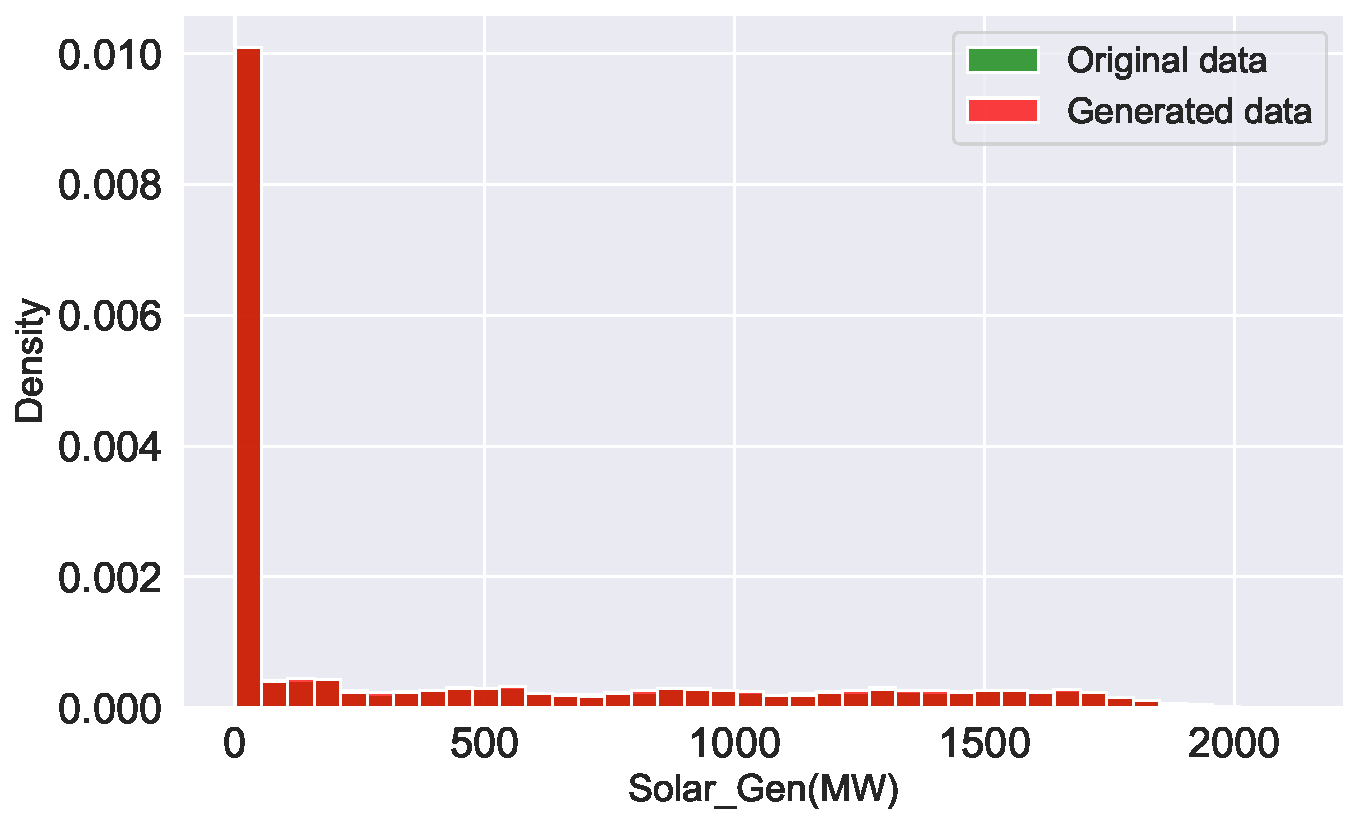
\includegraphics[width=\textwidth]{Figures/ProdCons/ProductionConsumption-Solar-HIST.pdf}
%          \caption{SolarGen}
%          \label{fig:SolarHist}
%     \end{subfigure}
%     \begin{subfigure}[b]{0.33\textwidth}
%          \centering
%          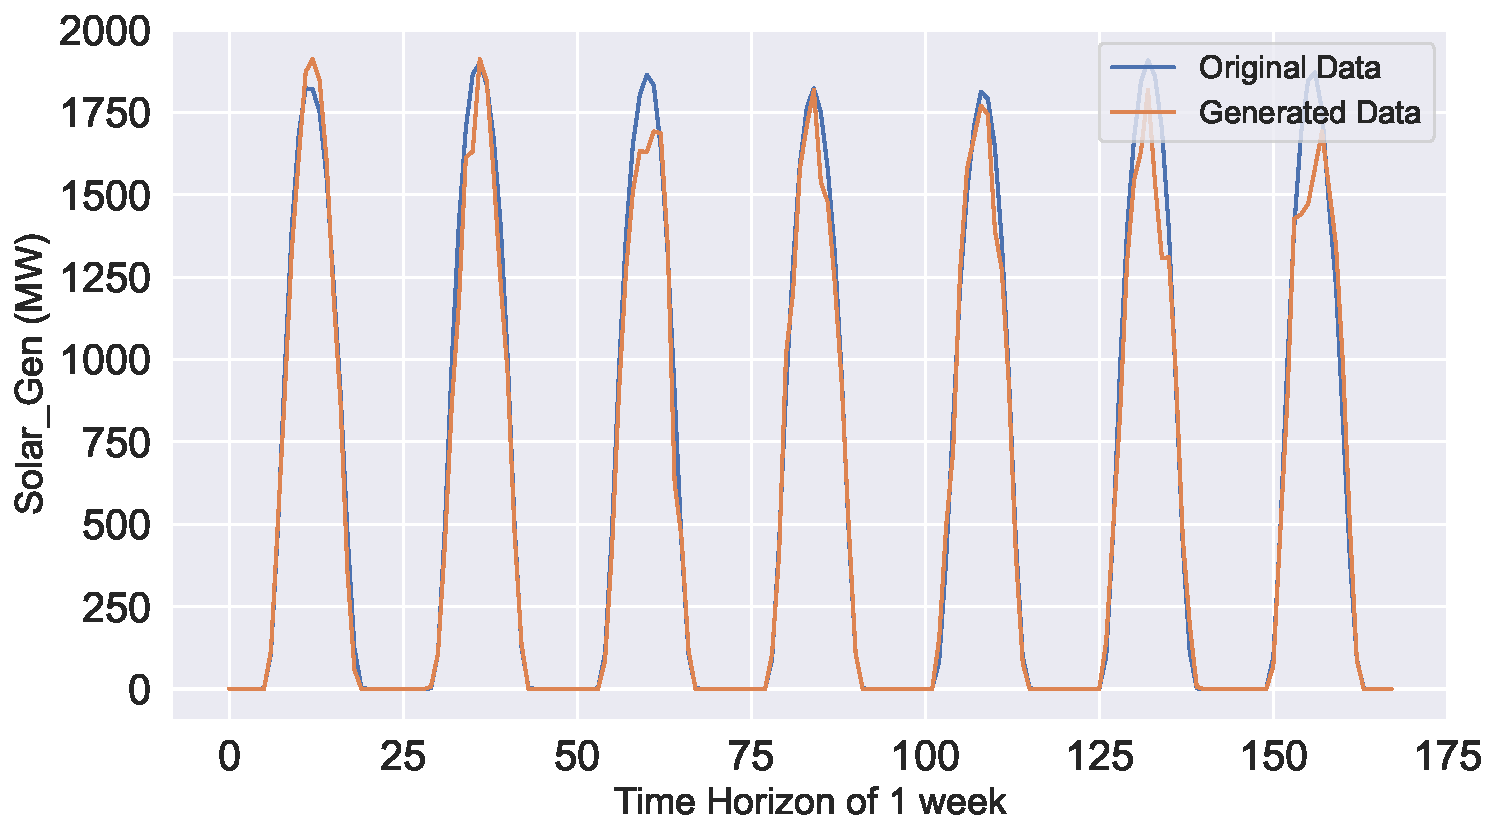
\includegraphics[width=\textwidth]{Figures/ProdCons/TimeSeries_Solar-HIST.pdf}
%          \caption{SolarGen}
%          \label{fig:SolarTimeSeries}
%      \end{subfigure}
    
    
%     \begin{subfigure}[b]{0.33\textwidth}
%          \centering
%          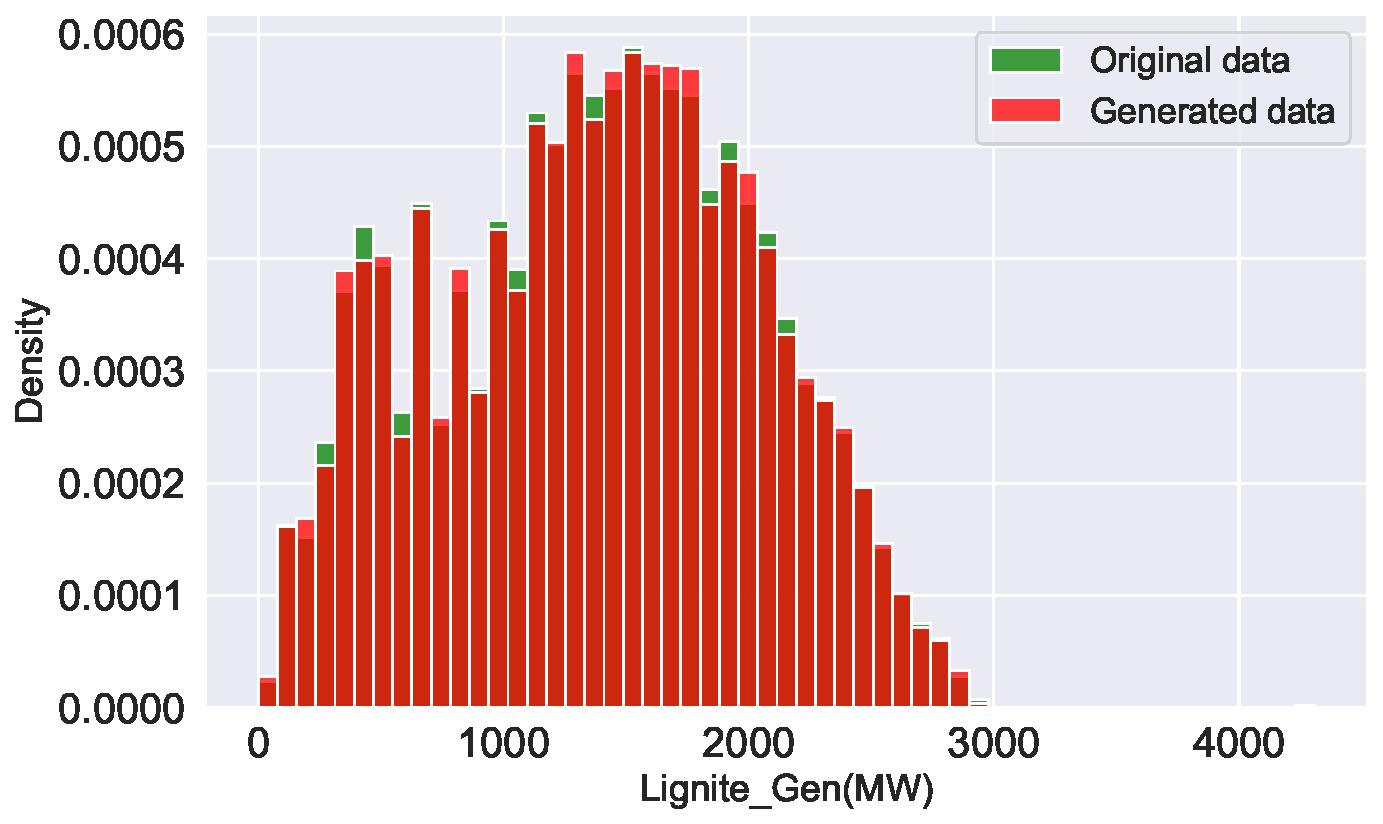
\includegraphics[width=\textwidth]{Figures/ProdCons/ProductionConsumption-Lignite-HIST.pdf}
%          \caption{LigniteGen}
%          \label{fig:LginteHist}
%      \end{subfigure}
%      \begin{subfigure}[b]{0.33\textwidth}
%          \centering
%          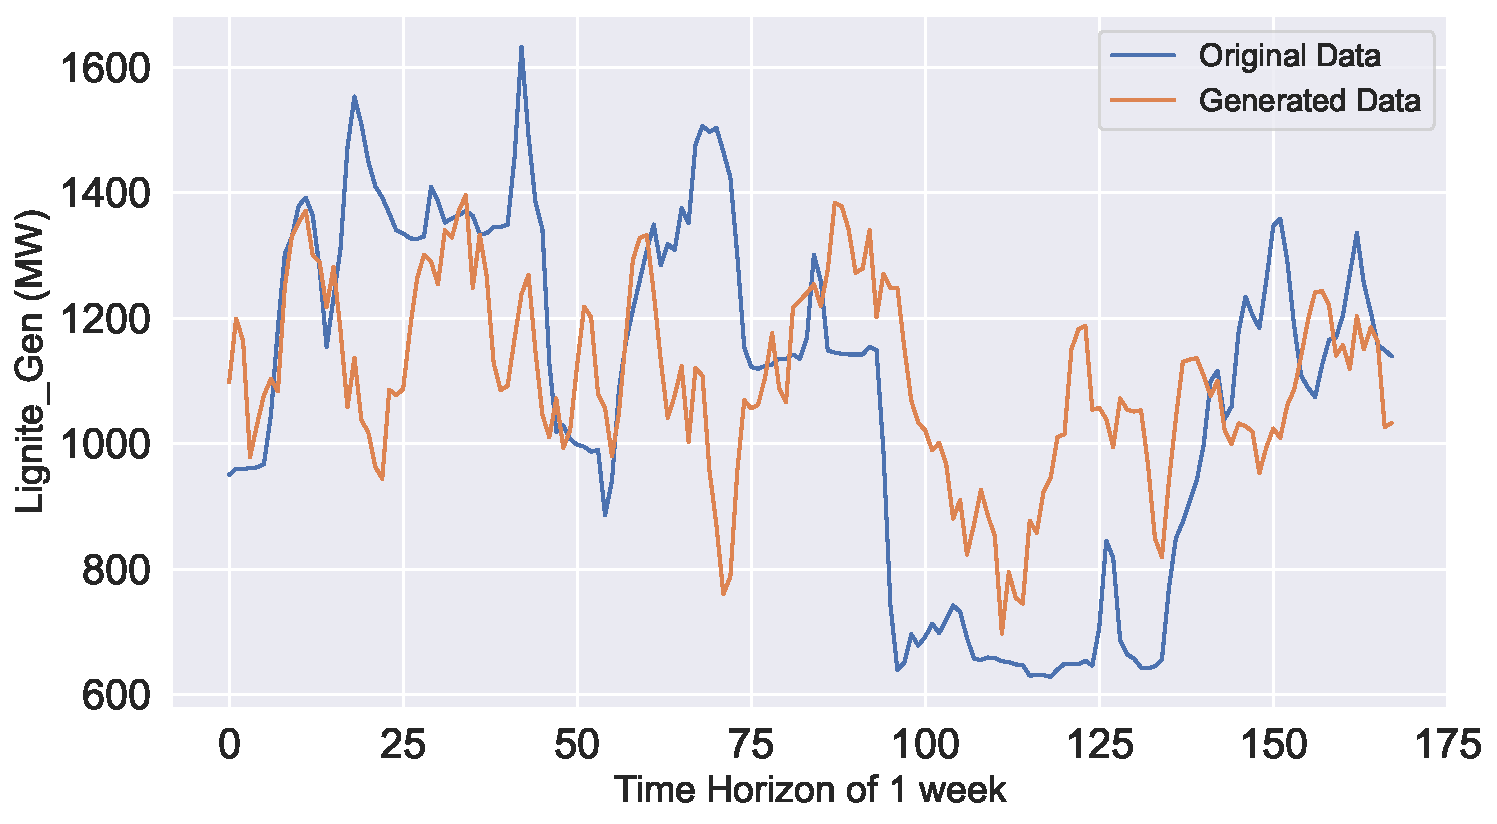
\includegraphics[width=\textwidth]{Figures/ProdCons/TimeSeries_Lignite-HIST.pdf}
%          \caption{LigniteGen-Smoothed, rolling window=12 hours}
%          \label{fig:LigniteTimeSeries}
%      \end{subfigure}
     
%     % \begin{subfigure}[b]{0.35\textwidth}
%     %      \centering
%     %      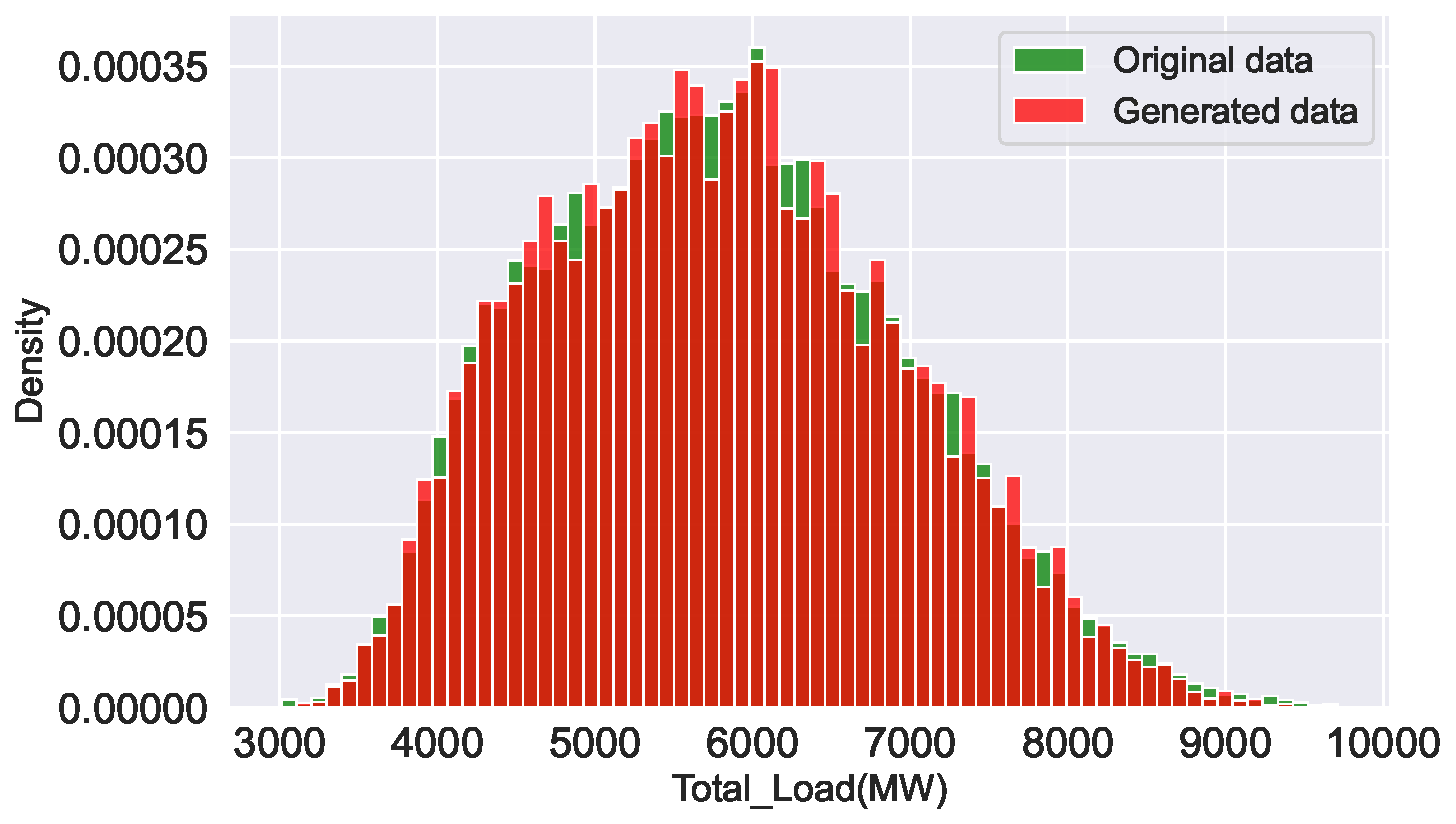
\includegraphics[width=\textwidth]{Figures/ProdCons/ProductionConsumption-TotalLoad-HIST.pdf}
%     %      \caption{Total\_Load}
%     %      \label{fig:totalLoad}
%     %  \end{subfigure}
%     % \begin{subfigure}[b]{0.35\textwidth}
%     %      \centering
%     %      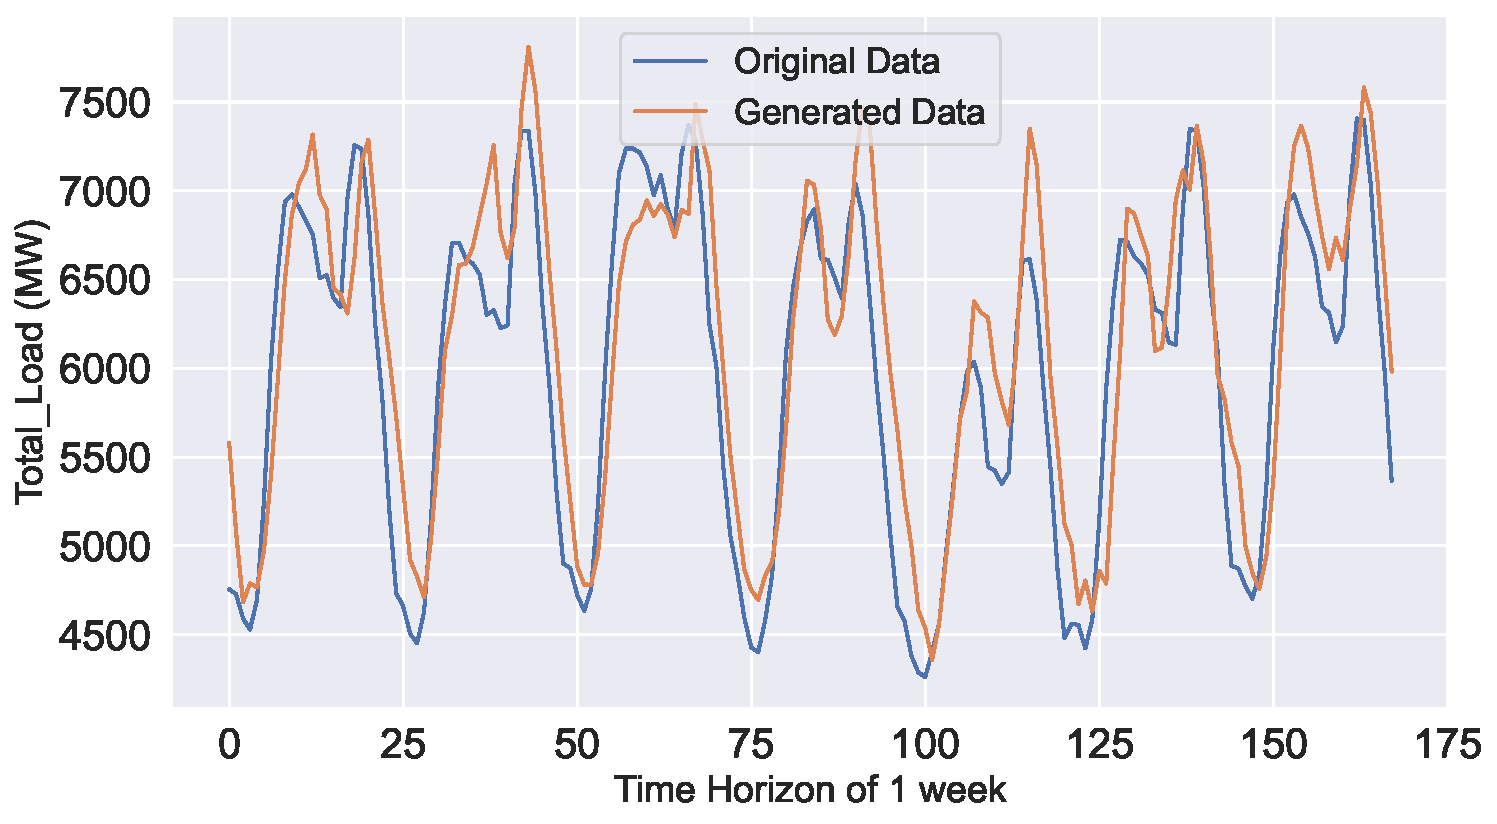
\includegraphics[width=\textwidth]{Figures/ProdCons/TimeSeries_TotalLoad-HIST.pdf}
%     %      \caption{Total\_Load-Smoothed,rolling=3}
%     %      \label{fig:LigniteTimeSeries}
%     %  \end{subfigure}
%      \caption{Histograms and Time-Series of Production and Consumption Data (HIST method)}
%     \label{fig:plotsProdCons}
%     \Description{The Histograms and Time-Series for each of the variables of the original and generated Energy Production and Consumption data, for HIST method.}
% \end{figure*}

% \begin{figure*}[]
%      \centering
%      \begin{subfigure}[b]{0.33\textwidth}
%          \centering
%          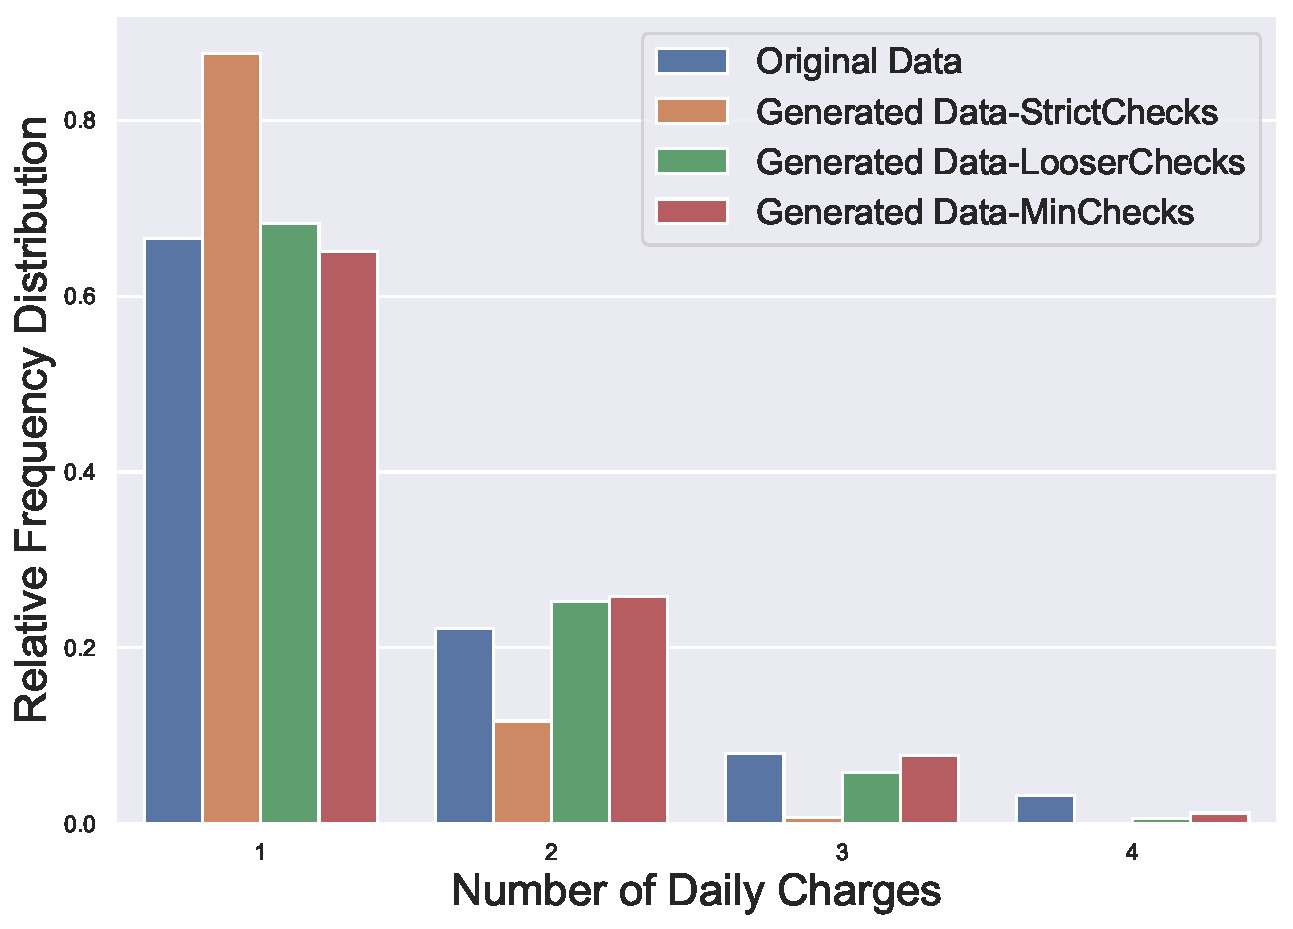
\includegraphics[width=\textwidth]{Figures/DriversBehavior/DriversBehavior_DailyCharges-ALL.pdf}
%          \caption{Daily Charges}
%          \label{fig:DailyCharges}
%      \end{subfigure}
%      \begin{subfigure}[b]{0.33\textwidth}
%          \centering
%          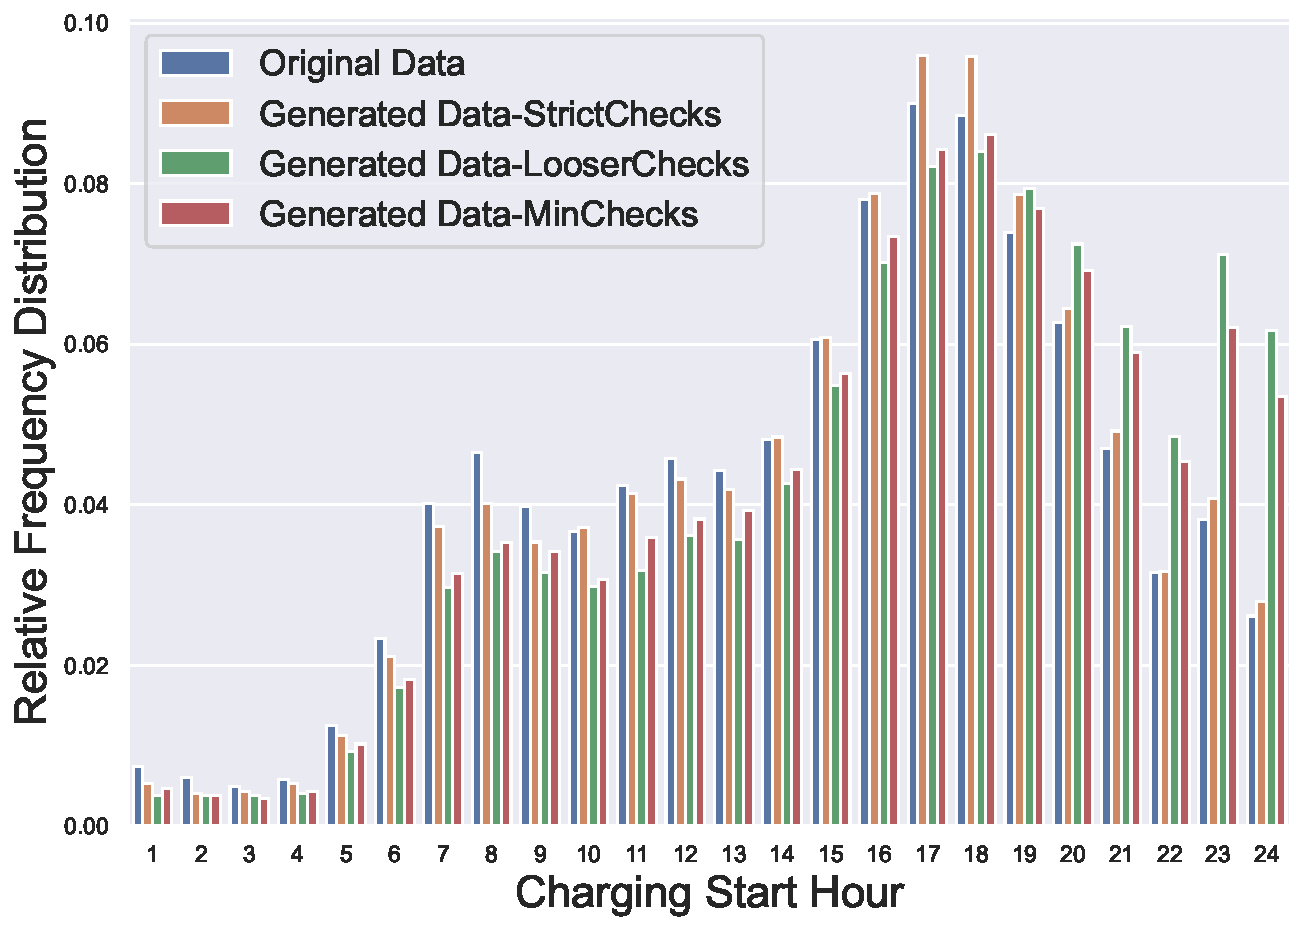
\includegraphics[width=\textwidth]{Figures/DriversBehavior/DriversBehavior_ChargeStartHour-ALL.pdf}
%          \caption{Charge Start Hour}
%          \label{fig:ChargeStartHours}
%      \end{subfigure}
     
%      \begin{subfigure}[b]{0.33\textwidth}
%          \centering
%          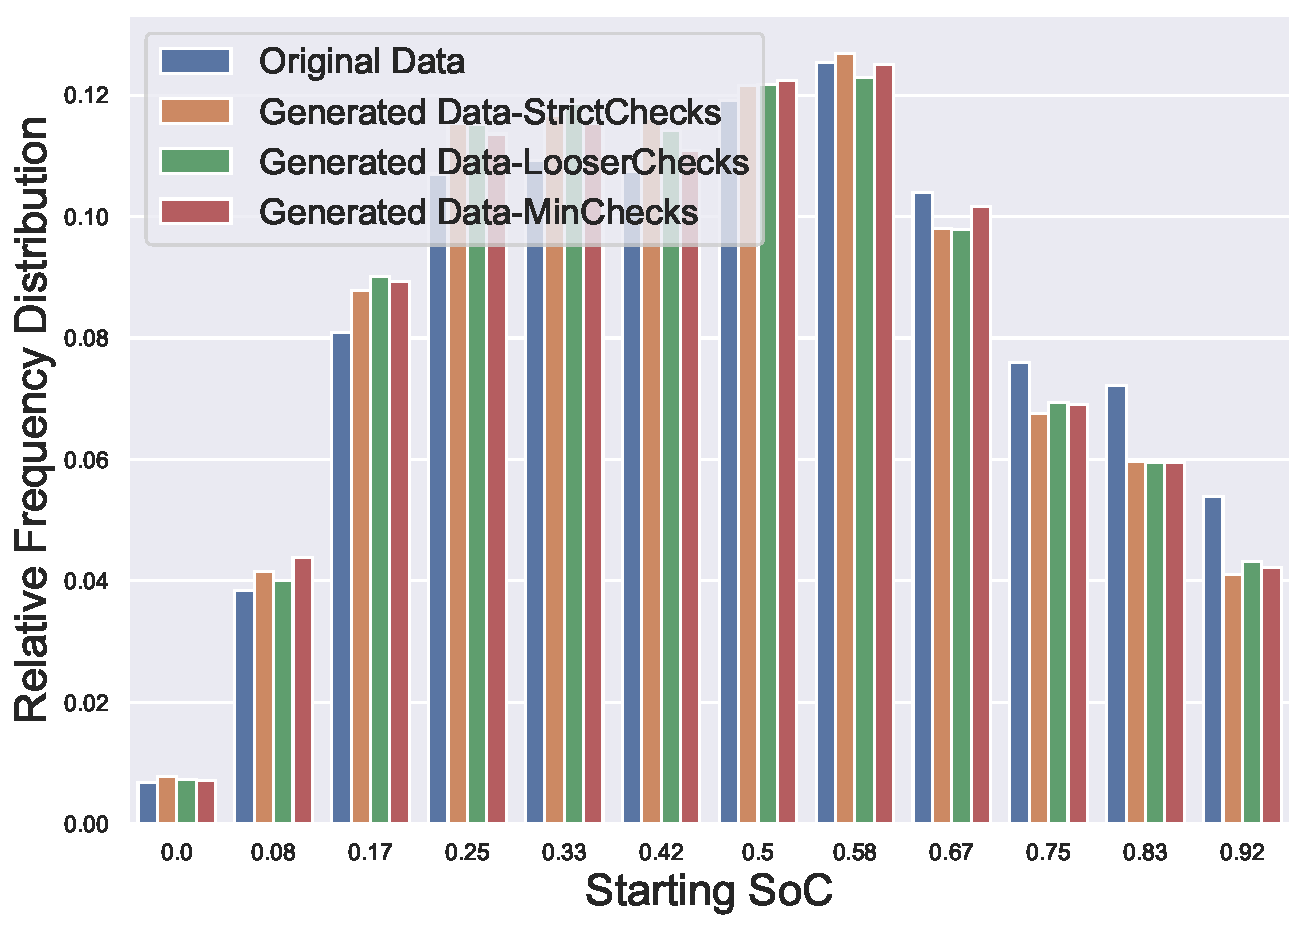
\includegraphics[width=\textwidth]{Figures/DriversBehavior/DriversBehavior_Starting_SoC-ALL.pdf}
%          \caption{Starting SoC}
%          \label{fig:StartingSoC}
%      \end{subfigure}
%      \begin{subfigure}[b]{0.33\textwidth}
%         \centering
%         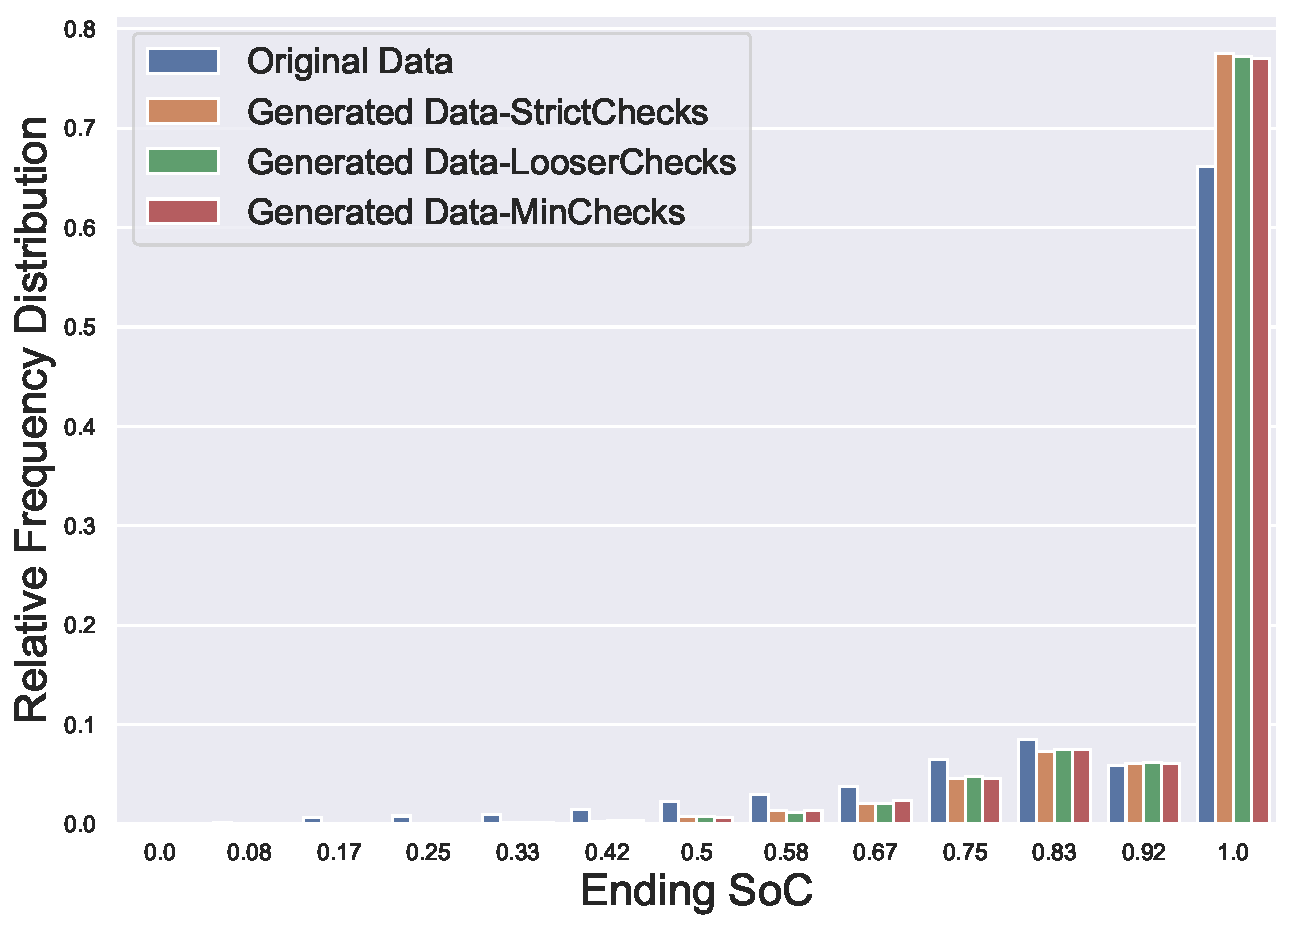
\includegraphics[width=\textwidth]{Figures/DriversBehavior/DriversBehavior_Ending_SoC-ALL.pdf}
%         \caption{Ending SoC}
%         \label{fig:EndingSoC}
%      \end{subfigure}
%     %  \begin{subfigure}[b]{0.3\textwidth}
%     %     \centering
%     %     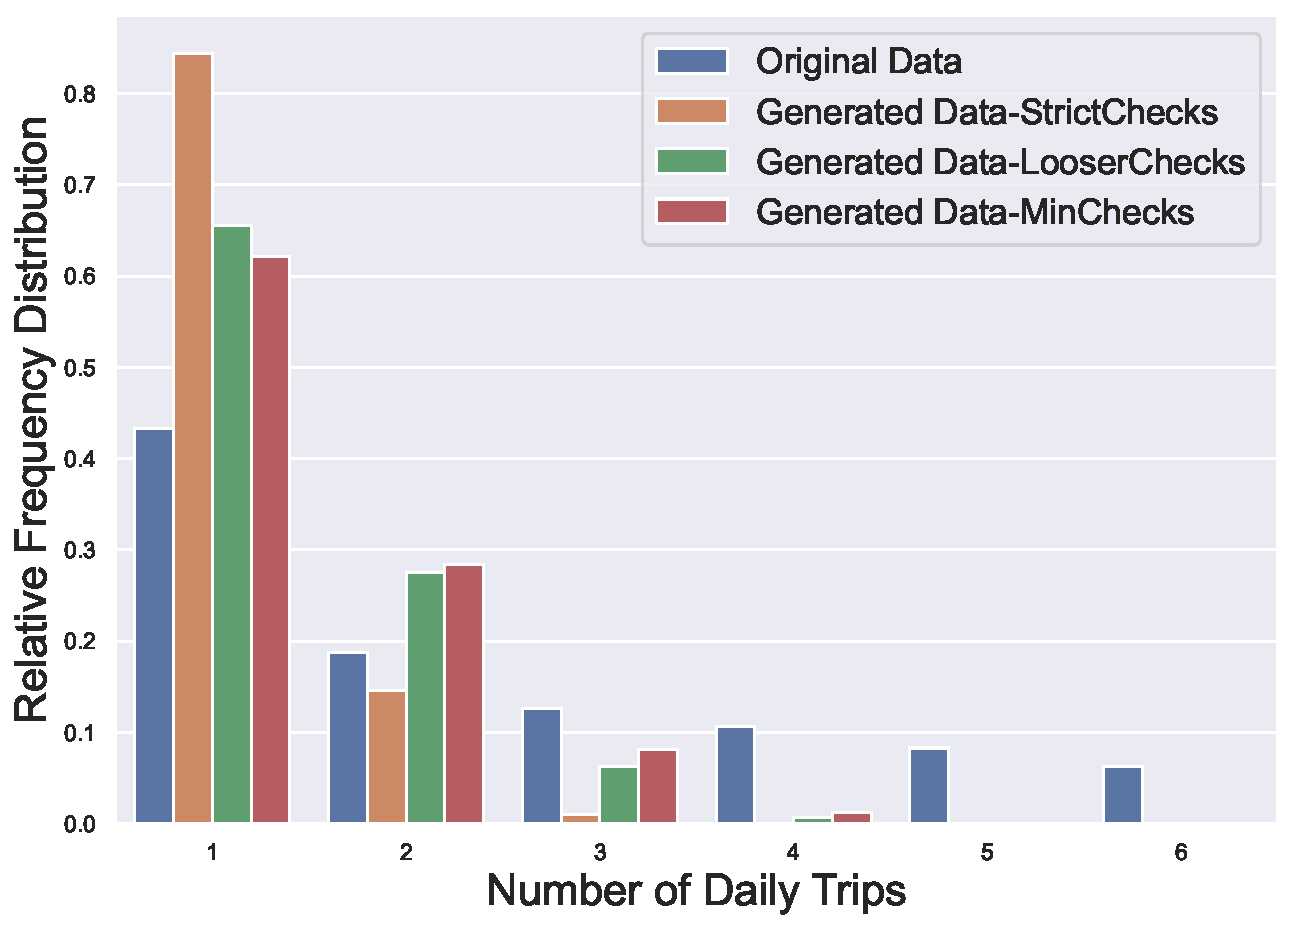
\includegraphics[width=\textwidth]{Figures/DriversBehavior/DriversBehavior_DailyTrips-ALL.pdf}
%     %     \caption{Daily Trips}
%     %     \label{fig:DailyTrips}
%     %  \end{subfigure}
%     %  \begin{subfigure}[b]{0.3\textwidth}
%     %     \centering
%     %     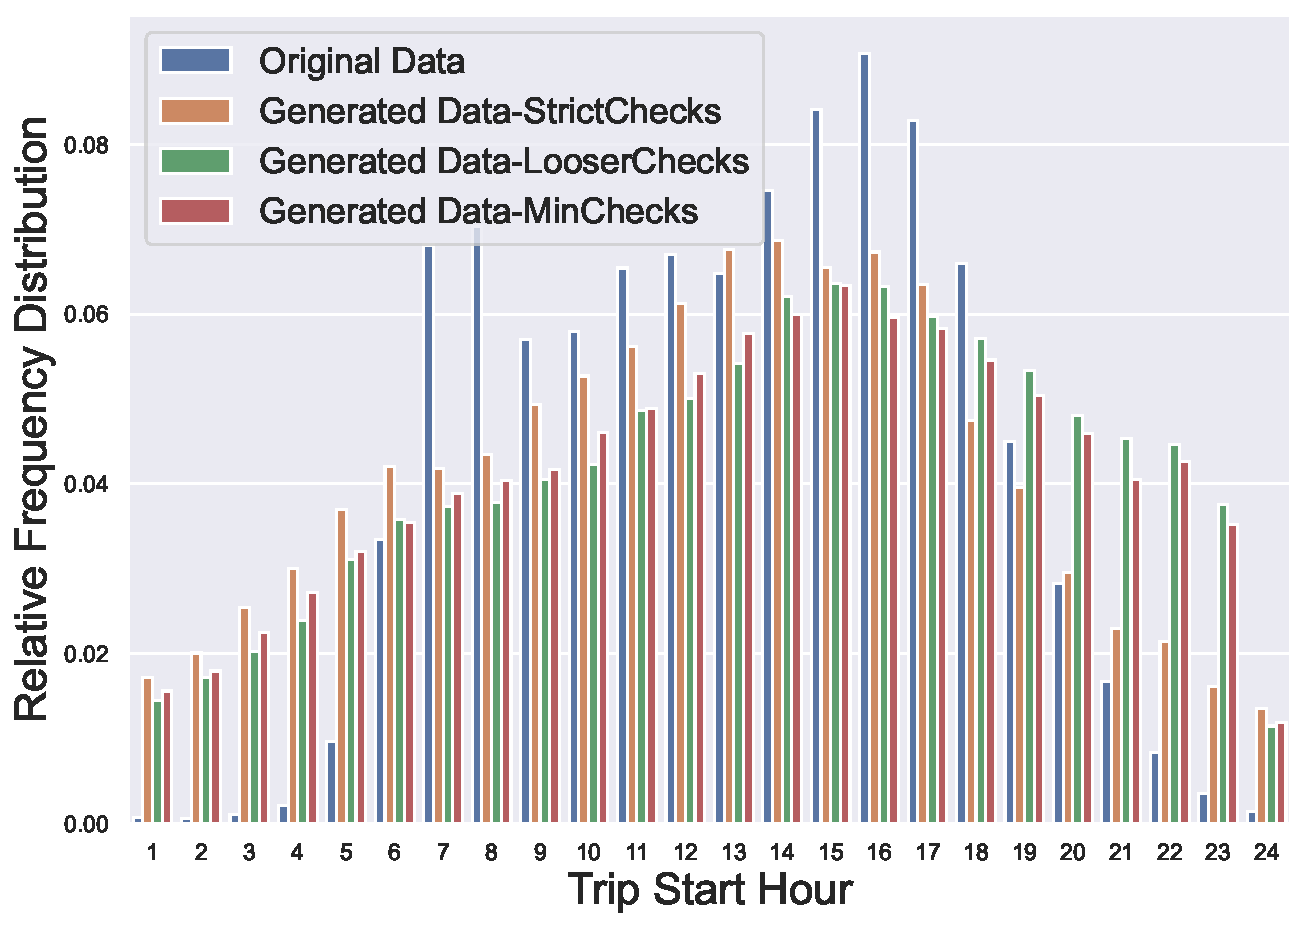
\includegraphics[width=\textwidth]{Figures/DriversBehavior/DriversBehavior_TripStartHour-ALL.pdf}
%     %     \caption{Trip Start Hour}
%     %     \label{fig:TripStartHour}
%     %  \end{subfigure}
%     \caption{Barplots of Drivers Behavior Frequency Tables}
%     \label{fig:plotsDrivBeh}
%     \Description{6 Figures-one for each variable- that show the Barplots for the Frequency Tables of the original and generated data. In each Figure the barplots of the original data are compared with those of the generated ones - for each of the 3 methods}
% \end{figure*}


% \begin{figure}
%      \centering
%      \begin{subfigure}[b]{0.37\textwidth}
%         \centering
%         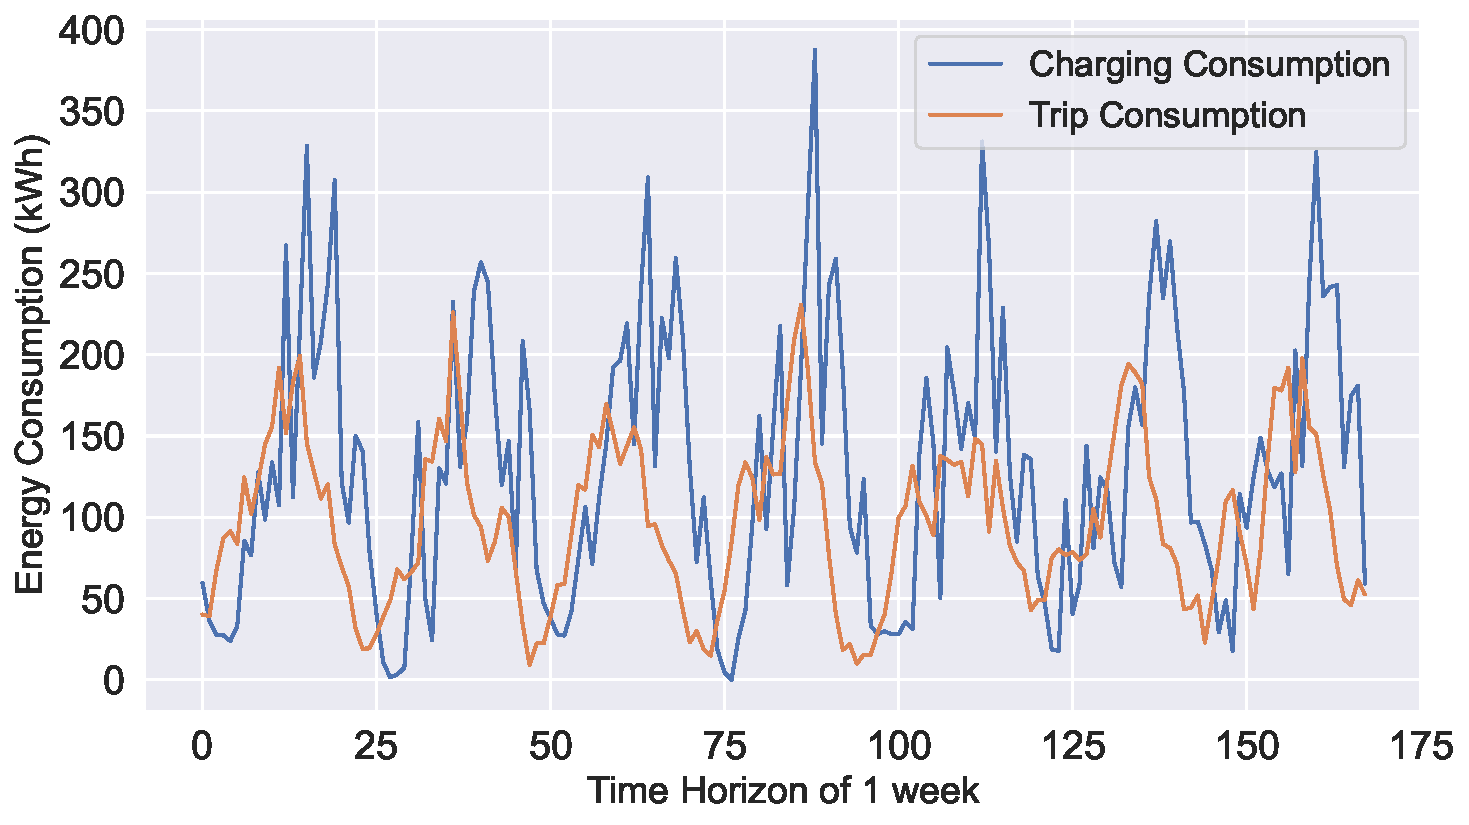
\includegraphics[width=\textwidth]{Figures/DriversBehavior/EVsConsumptions-StrictChecks.pdf}
%         \caption{Strict Checks}
%         \label{fig:TimeStrictChecks}
%      \end{subfigure}
%      \begin{subfigure}[b]{0.37\textwidth}
%         \centering
%         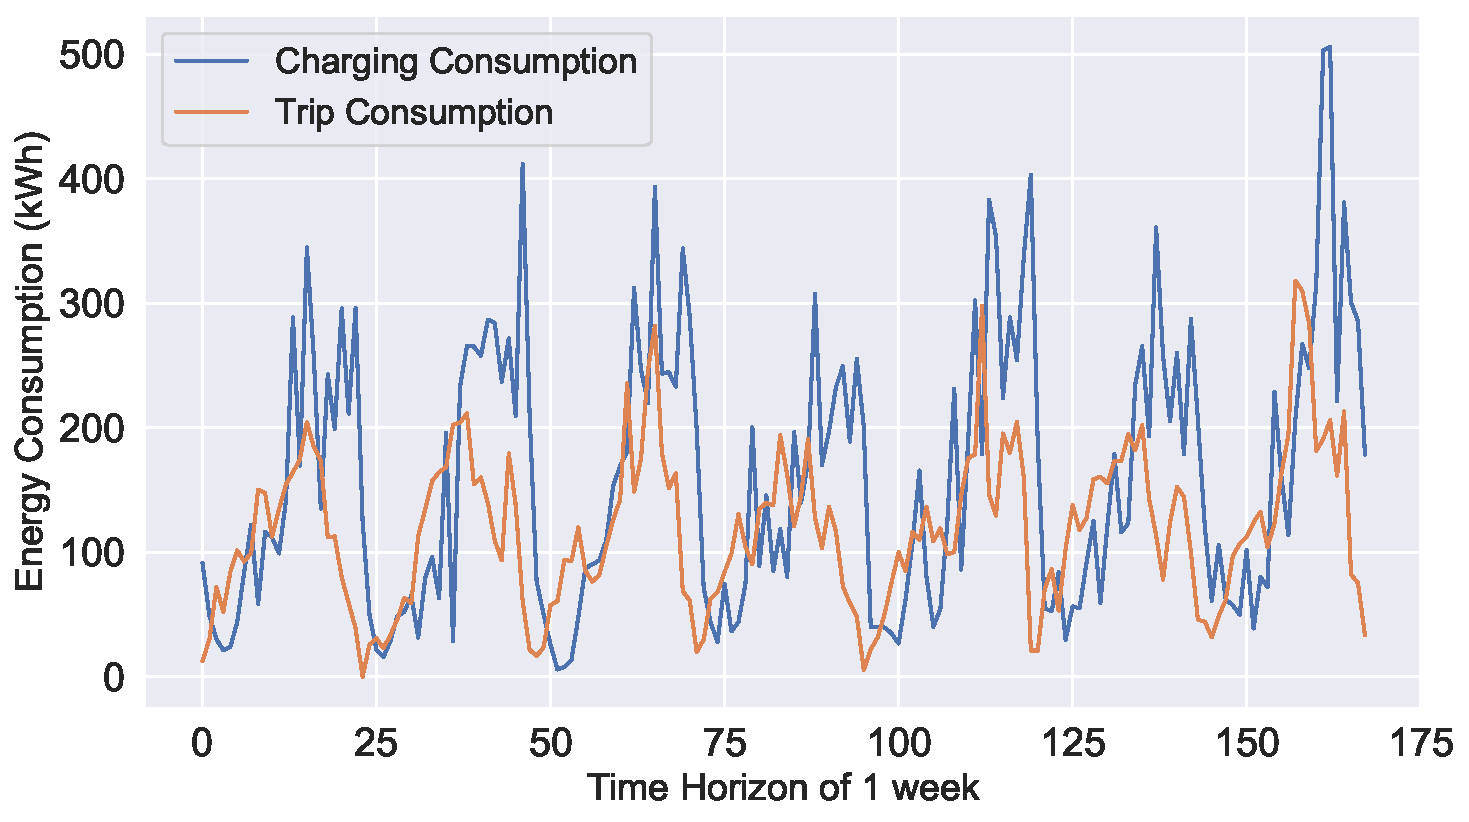
\includegraphics[width=\textwidth]{Figures/DriversBehavior/EVsConsumptions-LooserChecks.pdf}
%         \caption{Looser Checks}
%         \label{fig:TimeLooserChecks}
%      \end{subfigure}
%      \begin{subfigure}[b]{0.37\textwidth}
%         \centering
%         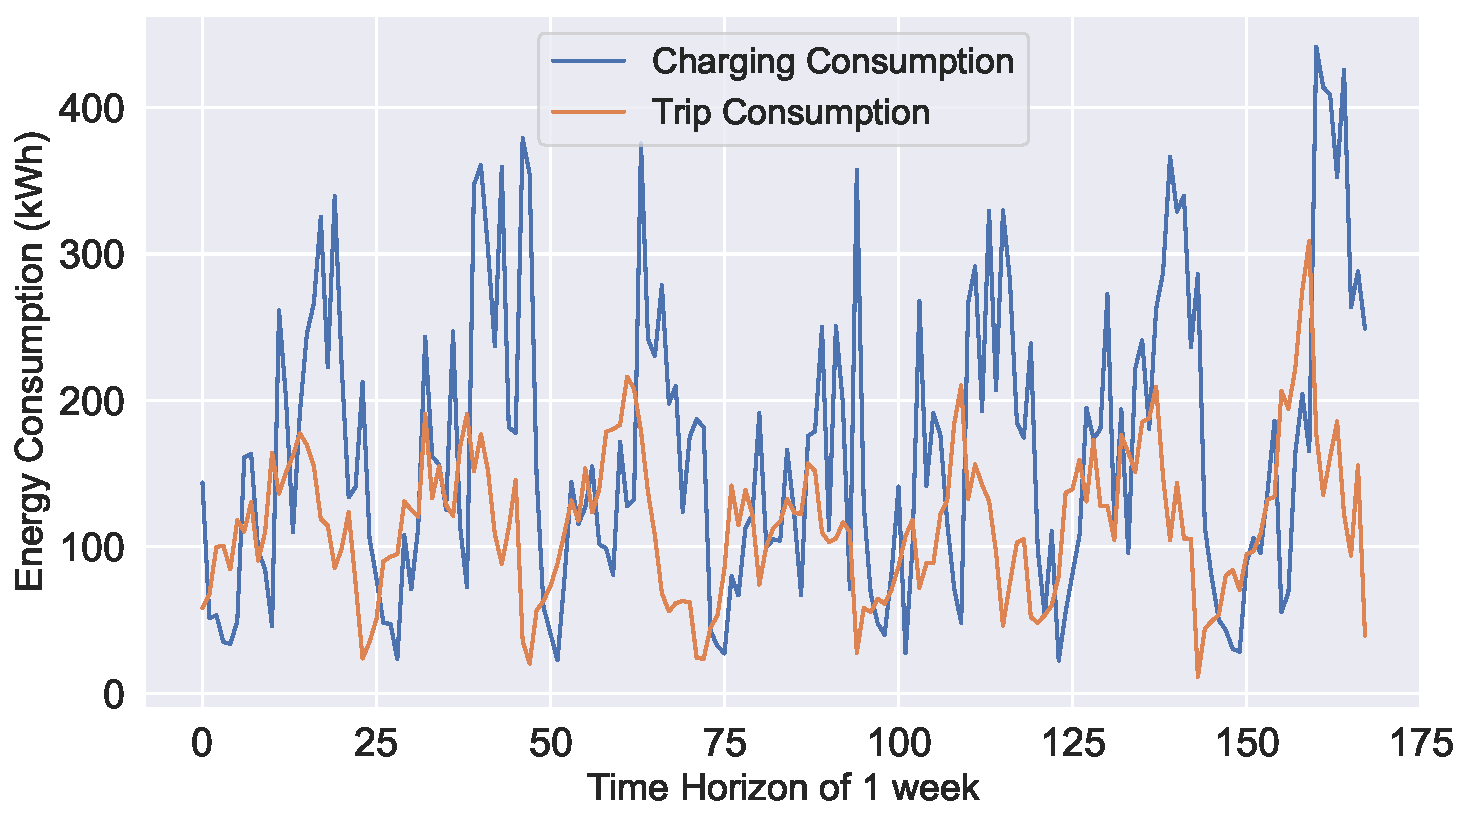
\includegraphics[width=\textwidth]{Figures/DriversBehavior/EVsConsumptions-MinChecks.pdf}
%         \caption{Min Checks}
%         \label{fig:TimeMinChecks}
%      \end{subfigure}
%     \caption{Time-Series of EVs Consumption  (Generated Data)}
%     \label{fig:TimeSeriesEVs}
%     \Description{3 figures (one for each method) that show the Time-Series of EV's energy consumption-while on trip and while charging-for the generated data, for a time horizon of 1 week.}
% \end{figure}

% %Regarding EVs and Drivers Behaviour data, the results presented in 
% Table~\ref{tab:metricsEV} summarizes the differences between the barplots of the original and generated EVs and Drivers' Behaviour data, 
% %are calculated from experiments 
% %with
% of 100 EVs in a time horizon of 1 year. The overall performance of \emph{MinChecks} mode appears to be better than the other two modes. The results interpretation is a bit more intricate, however. %However, by observing each variable/column individually, we realize that the results intepretation is a  
 
% First, the column \emph{DailyCharges} has the largest difference between the original-generated data for the \emph{StrictChecks} method and the smallest for the \emph{MinChecks} method. This is also illustrated in Fig.~\ref{fig:plotsDrivBeh}: in the \emph{StrictChecks} mode we have mainly 1 to 2 charges, in rare cases 3 and very rarely 4 charges, while for \emph{LooserChecks} and \emph{MinChecks} the number of total daily charges is distributed similarly to the original data.
% The specific results are meaningful, considering that in the \emph{StrictChecks} mode, we first visit a number of constraints regarding the number of charges. As mentioned in Section~\ref{subsec:dribehgen}, in order for the next charge to take place, the previous one must have been completed at a certain time point during the day. Conversely, in the \emph{LooserChecks} mode, the only check that is done before attempting the next charge is that the previous one has to be completed before 23:00 on the same day, while in \emph{MinChecks} no check is performed. Consequently, 
% %with respect to daily charges, 
% the more constraints we apply {\em wrt} 
% %daily 
% charges--i.e., the narrower the time period during which a charge can be made--the fewer charges will be performed daily.
% %during the day.
% % It therefore makes sense that the \emph{MinChecks} mode has the best performance, while \emph{StrictChecks} mode has the worst.

% At the same time, however, the strict constraints of the first method give us better control over the variables \emph{ChargeStartHour} and \emph{TripStartHour} and therefore optimize the results for the respective columns, while all three modes have similar performance with respect to the \emph{StartingSoC} and the \emph{EndingSoC} variables.


% % {\color{red} Also, due to the direct dependence of daily trips with daily charges,\footnote{Recall that we first sample the number of daily charges, and then fill the trip number and details, as inferred from the sampled charges.}
% % the smaller the number of daily charges, the fewer daily trips will be performed.
% % Considering that in the generated data we mainly produce 1-2 daily charges, sometimes 3 and fewer times 4,
% % then, respectively, only 1 or 2 daily trips will be generated, fewer times 3 and very rarely 4 or more. Due to this, the daily trips generated distributions that are quite different than the original one (see Table~\ref{tab:metricsEV} and Figure~\ref{fig:DailyTrips}).}


% Finally, Figure~\ref{fig:TimeSeriesEVs} shows the total energy consumption during charging and trip events of 100 EVs for a time horizon of 1 week, generated by each one of the 3 modes. We observe a phase difference between Charging and Trip Consumption, which makes sense, as a vehicle cannot charge its battery at a charging station and travel at the same time. In addition, we notice that there are energy losses, as expected due to several factors: 
% %the electrical power 
% AC to DC conversion,
% %the AC supply to the DC Li-ion battery 
% %(up to 5\% loses for  11 kW AC power~\cite{apostolaki2017measurement}), 
% wiring losses, 
% %several 
% %undesired 
% internal electrochemical reactions, %inadequate operation of the BMS 
% battery management system malfunctions,
% and cell warming due to internal resistance~\cite{dai2013cell,kostopoulos2020real}.
% %Note also that in our data (both the original and, thus, the generated), the majority of drivers, fully charge their EV battery at each charge (Figure~\ref{fig:EndingSoC}); 
% %then since charging continues beyond 80\% of SoC, 
% %as such, losses are 
% %almost double compared to those anticipated had the SoC been maintained within the 20\%–80\% of capacity~\cite{kostopoulos2020real}.   %%At this point we can not omit the regenerative braking factor. 
% %Regenerative braking, %%is a process 
% %where during the trip an amount of energy is going into the battery, % and therefore we have partial energy recovery
% %is also a factor contributing to these results~\cite{de2015electric}.
% %%%%%%%%%%%%%%%%%%%%%%%%%%%%%%%%%%%%%%%%%%%%%%%%%%%%%%%%%%%%%%%%%%%%%%%%%%%%%%%%%%%%%%
% \subsection{Discussion}
% \label{sec:discussion}
% %By the general figure of the statistics presented above, it appears 
% Our results above show that in cases where we create a relatively large number of Production and Consumption data using the KDE and Histogram sampling methods, the overall picture of the generated data is very close to the original. However, for specific types of data (e.g., in the case of Lignite generation) that exhibit no periodicity, we see that the methods tested are less effective in producing similar time series patterns as the original data.\footnote{Of course, it has to be noted that a perfect match is in many cases not desirable, due to privacy-related concerns.}  In addition, we report that the TimeGAN method, despite its positive evaluation in the literature~\cite{yoon2019time}, which was the motivating factor for including it in our current implementation, generates time series whose patterns are quite different than the ones in the original data for all generated variable types.

% %Nevertheless, the proposed 
% We note that our dataset generator can be used for the verification of multiagent systems and other G2V/V2G approaches. The heterogeneity of such models and related environments implies dynamic changes and fluctuations in the various measurements and exchanged values. Thus, to make sure that an experimental approach is robust and resilient in various application sites, it is crucial to test it using a number of different datasets, with varying, yet realistic behaviors, which is often very hard to obtain. Also, datasets that have a different form with respect to their time series patterns, but follow similar models, are also of interest, since they can be used to examine attack patterns and mitigations, among other security issues. To the best of our knowledge, not much related research exists, and we believe that the proposed dataset generator constitutes a valuable tool for this domain of research too.




% %%%%%%%%%%%%%%%%%%%%%%%%%%%%%%%%%%%%%%%%%%%%%%%%%%%%%%%%%%%%%%%%%%%%%%%%%%%%%%%%%%%%%%
% \section{Conclusions \& Future Work}
% \label{sec:con}

% %The EVs sector has been evolving dramatically the last decade and the existance of efficient algorithms that will be able to manage different EV activities is crucial. However, the development and evaluation of such algorithms frequently depends on the availability of large datasets. Such datasets, though, are usually either not large enough, or not freely available. Thus, 
% This paper addresses a pressing problem and need in the Smart Grid, via developing a dataset generator for EVs charging management. %in Smart Grids. 
% Our generator takes as input several publicly available datasets which contain data that describe different energy generation and demand types, as well as charging profiles of EVs and corresponding trip and type information. It then fits Histograms, Kernel Density Estimates, Generative Adversarial Networks, and Frequency Tables using the predifned data as training sets. Finally, it generates new synthetic data, which is not identical to the input, but adheres to the same principles, and relationships. The generator also accompanies the output datasets with corresponding summarizations, useful for detecting consistency issues. Our dataset generator will be made freely available for further evaluation and use by the community. 


% In terms of future work, we aim to evaluate the application of additional data analysis techniques for datasets  that exhibit some periodicity in their values; and at the same time, to explore ways to more accurately simulate data that does not appear to be periodic.
% %such as wind generation. 
% Additionally, apart from its main function, our dataset generator could also serve as a tool towards the verifiability of various multiagent systems, as explained in our discussion in Section~\ref{sec:discussion}.
% Finally, we intend to extend our dataset generator to cover the V2G mode of EV operation, which is crucial for the efficient integration of renewables into the Grid.


%%%%%%%%%%%%%%%%%%%%%%%%%%%%%%%%%%%%%%%%%%%%%%%%%%%%%%%%%%%%%%%%%%%%%%%%%%%%%%%%%%%%%%
%%%%%%%%%%%%%%%%%%%%%%%%%%%%%%%%%%%%%%%%%%%%%%%%%%%%%%%%%%%%%%%%%%%%%%%%%%%%%%%%%%%%%%
%%%%%%%%%%%%%%%%%%%%%%%%%%%%%%%%%%%%%%%%%%%%%%%%%%%%%%%%%%%%%%%%%%%%%%%%%%%%%%%%%%%%%%
%%%%%%%%%%%%%%%%%%%%%%%%%%%%%%%%%%%%%%%%%%%%%%%%%%%%%%%%%%%%%%%%%%%%%%%%%%%%%%%%%%%%%%
% \section{Authors and Affiliations}

% Each author must be defined separately for accurate metadata
% identification. Multiple authors may share one affiliation. Authors'
% names should not be abbreviated; use full first names wherever
% possible. Include authors' e-mail addresses whenever possible.

% Grouping authors' names or e-mail addresses, or providing an ``e-mail
% alias,'' as shown below, is not acceptable:
% \begin{verbatim}
%   \author{Brooke Aster, David Mehldau}
%   \email{dave,judy,steve@university.edu}
%   \email{firstname.lastname@phillips.org}
% \end{verbatim}

% The \verb|authornote| and \verb|authornotemark| commands allow a note
% to apply to multiple authors --- for example, if the first two authors
% of an article contributed equally to the work.

% If your author list is lengthy, you must define a shortened version of
% the list of authors to be used in the page headers, to prevent
% overlapping text. The following command should be placed just after
% the last \verb|\author{}| definition:
% \begin{verbatim}
%   \renewcommand{\shortauthors}{McCartney, et al.}
% \end{verbatim}
% Omitting this command will force the use of a concatenated list of all
% of the authors' names, which may result in overlapping text in the
% page headers.

% The article template's documentation, available at
% \url{https://www.acm.org/publications/proceedings-template}, has a
% complete explanation of these commands and tips for their effective
% use.

% Note that authors' addresses are mandatory for journal articles.

% \section{Rights Information}

% Authors of any work published by ACM will need to complete a rights
% form. Depending on the kind of work, and the rights management choice
% made by the author, this may be copyright transfer, permission,
% license, or an OA (open access) agreement.

% Regardless of the rights management choice, the author will receive a
% copy of the completed rights form once it has been submitted. This
% form contains \LaTeX\ commands that must be copied into the source
% document. When the document source is compiled, these commands and
% their parameters add formatted text to several areas of the final
% document:
% \begin{itemize}
% \item the ``ACM Reference Format'' text on the first page.
% \item the ``rights management'' text on the first page.
% \item the conference information in the page header(s).
% \end{itemize}

% Rights information is unique to the work; if you are preparing several
% works for an event, make sure to use the correct set of commands with
% each of the works.

% The ACM Reference Format text is required for all articles over one
% page in length, and is optional for one-page articles (abstracts).

% \section{CCS Concepts and User-Defined Keywords}

% Two elements of the ``acmart'' document class provide powerful
% taxonomic tools for you to help readers find your work in an online
% search.

% The ACM Computing Classification System ---
% \url{https://www.acm.org/publications/class-2012} --- is a set of
% classifiers and concepts that describe the computing
% discipline. Authors can select entries from this classification
% system, via \url{https://dl.acm.org/ccs/ccs.cfm}, and generate the
% commands to be included in the \LaTeX\ source.

% User-defined keywords are a comma-separated list of words and phrases
% of the authors' choosing, providing a more flexible way of describing
% the research being presented.

% CCS concepts and user-defined keywords are required for for all
% articles over two pages in length, and are optional for one- and
% two-page articles (or abstracts).

% \section{Sectioning Commands}

% Your work should use standard \LaTeX\ sectioning commands:
% \verb|section|, \verb|subsection|, \verb|subsubsection|, and
% \verb|paragraph|. They should be numbered; do not remove the numbering
% from the commands.

% Simulating a sectioning command by setting the first word or words of
% a paragraph in boldface or italicized text is {\bfseries not allowed.}

% \section{Tables}

% The ``\verb|acmart|'' document class includes the ``\verb|booktabs|''
% package --- \url{https://ctan.org/pkg/booktabs} --- for preparing
% high-quality tables.

% Table captions are placed {\itshape above} the table.

% Because tables cannot be split across pages, the best placement for
% them is typically the top of the page nearest their initial cite.  To
% ensure this proper ``floating'' placement of tables, use the
% environment \textbf{table} to enclose the table's contents and the
% table caption.  The contents of the table itself must go in the
% \textbf{tabular} environment, to be aligned properly in rows and
% columns, with the desired horizontal and vertical rules.  Again,
% detailed instructions on \textbf{tabular} material are found in the
% \textit{\LaTeX\ User's Guide}.

% Immediately following this sentence is the point at which
% Table~\ref{tab:freq} is included in the input file; compare the
% placement of the table here with the table in the printed output of
% this document.

% \begin{table}
%   \caption{Frequency of Special Characters}
%   \label{tab:freq}
%   \begin{tabular}{ccl}
%     \toprule
%     Non-English or Math&Frequency&Comments\\
%     \midrule
%     \O & 1 in 1,000& For Swedish names\\
%     $\pi$ & 1 in 5& Common in math\\
%     \$ & 4 in 5 & Used in business\\
%     $\Psi^2_1$ & 1 in 40,000& Unexplained usage\\
%   \bottomrule
% \end{tabular}
% \end{table}

% To set a wider table, which takes up the whole width of the page's
% live area, use the environment \textbf{table*} to enclose the table's
% contents and the table caption.  As with a single-column table, this
% wide table will ``float'' to a location deemed more
% desirable. Immediately following this sentence is the point at which
% Table~\ref{tab:commands} is included in the input file; again, it is
% instructive to compare the placement of the table here with the table
% in the printed output of this document.

% \begin{table*}
%   \caption{Some Typical Commands}
%   \label{tab:commands}
%   \begin{tabular}{ccl}
%     \toprule
%     Command &A Number & Comments\\
%     \midrule
%     \texttt{{\char'134}author} & 100& Author \\
%     \texttt{{\char'134}table}& 300 & For tables\\
%     \texttt{{\char'134}table*}& 400& For wider tables\\
%     \bottomrule
%   \end{tabular}
% \end{table*}

% Always use midrule to separate table header rows from data rows, and
% use it only for this purpose. This enables assistive technologies to
% recognise table headers and support their users in navigating tables
% more easily.

% \section{Math Equations}
% You may want to display math equations in three distinct styles:
% inline, numbered or non-numbered display.  Each of the three are
% discussed in the next sections.

% \subsection{Inline (In-text) Equations}
% A formula that appears in the running text is called an inline or
% in-text formula.  It is produced by the \textbf{math} environment,
% which can be invoked with the usual
% \texttt{{\char'134}begin\,\ldots{\char'134}end} construction or with
% the short form \texttt{\$\,\ldots\$}. You can use any of the symbols
% and structures, from $\alpha$ to $\omega$, available in
% \LaTeX~\cite{Lamport:LaTeX}; this section will simply show a few
% examples of in-text equations in context. Notice how this equation:
% \begin{math}
%   \lim_{n\rightarrow \infty}x=0
% \end{math},
% set here in in-line math style, looks slightly different when
% set in display style.  (See next section).

% \subsection{Display Equations}
% A numbered display equation---one set off by vertical space from the
% text and centered horizontally---is produced by the \textbf{equation}
% environment. An unnumbered display equation is produced by the
% \textbf{displaymath} environment.

% Again, in either environment, you can use any of the symbols and
% structures available in \LaTeX\@; this section will just give a couple
% of examples of display equations in context.  First, consider the
% equation, shown as an inline equation above:
% \begin{equation}
%   \lim_{n\rightarrow \infty}x=0
% \end{equation}
% Notice how it is formatted somewhat differently in
% the \textbf{displaymath}
% environment.  Now, we'll enter an unnumbered equation:
% \begin{displaymath}
%   \sum_{i=0}^{\infty} x + 1
% \end{displaymath}
% and follow it with another numbered equation:
% \begin{equation}
%   \sum_{i=0}^{\infty}x_i=\int_{0}^{\pi+2} f
% \end{equation}
% just to demonstrate \LaTeX's able handling of numbering.

% \section{Figures}

% The ``\verb|figure|'' environment should be used for figures. One or
% more images can be placed within a figure. If your figure contains
% third-party material, you must clearly identify it as such, as shown
% in the example below.
% \begin{figure}[h]
%   \centering
%   \includegraphics[width=\linewidth]{sample-franklin}
%   \caption{1907 Franklin Model D roadster. Photograph by Harris \&
%     Ewing, Inc. [Public domain], via Wikimedia
%     Commons. (\url{https://goo.gl/VLCRBB}).}
%   \Description{A woman and a girl in white dresses sit in an open car.}
% \end{figure}

% Your figures should contain a caption which describes the figure to
% the reader.

% Figure captions are placed {\itshape below} the figure.

% Every figure should also have a figure description unless it is purely
% decorative. These descriptions convey what’s in the image to someone
% who cannot see it. They are also used by search engine crawlers for
% indexing images, and when images cannot be loaded.

% A figure description must be unformatted plain text less than 2000
% characters long (including spaces).  {\bfseries Figure descriptions
%   should not repeat the figure caption – their purpose is to capture
%   important information that is not already provided in the caption or
%   the main text of the paper.} For figures that convey important and
% complex new information, a short text description may not be
% adequate. More complex alternative descriptions can be placed in an
% appendix and referenced in a short figure description. For example,
% provide a data table capturing the information in a bar chart, or a
% structured list representing a graph.  For additional information
% regarding how best to write figure descriptions and why doing this is
% so important, please see
% \url{https://www.acm.org/publications/taps/describing-figures/}.

% \subsection{The ``Teaser Figure''}

% A ``teaser figure'' is an image, or set of images in one figure, that
% are placed after all author and affiliation information, and before
% the body of the article, spanning the page. If you wish to have such a
% figure in your article, place the command immediately before the
% \verb|\maketitle| command:
% \begin{verbatim}
%   \begin{teaserfigure}
%     \includegraphics[width=\textwidth]{sampleteaser}
%     \caption{figure caption}
%     \Description{figure description}
%   \end{teaserfigure}
% \end{verbatim}

% \section{Citations and Bibliographies}

% The use of \BibTeX\ for the preparation and formatting of one's
% references is strongly recommended. Authors' names should be complete
% --- use full first names (``Donald E. Knuth'') not initials
% (``D. E. Knuth'') --- and the salient identifying features of a
% reference should be included: title, year, volume, number, pages,
% article DOI, etc.

% The bibliography is included in your source document with these two
% commands, placed just before the \verb|\end{document}| command:
% \begin{verbatim}
%   \bibliographystyle{ACM-Reference-Format}
%   \bibliography{bibfile}
% \end{verbatim}
% where ``\verb|bibfile|'' is the name, without the ``\verb|.bib|''
% suffix, of the \BibTeX\ file.

% Citations and references are numbered by default. A small number of
% ACM publications have citations and references formatted in the
% ``author year'' style; for these exceptions, please include this
% command in the {\bfseries preamble} (before the command
% ``\verb|\begin{document}|'') of your \LaTeX\ source:
% \begin{verbatim}
%   \citestyle{acmauthoryear}
% \end{verbatim}

%   Some examples.  A paginated journal article \cite{Abril07}, an
%   enumerated journal article \cite{Cohen07}, a reference to an entire
%   issue \cite{JCohen96}, a monograph (whole book) \cite{Kosiur01}, a
%   monograph/whole book in a series (see 2a in spec. document)
%   \cite{Harel79}, a divisible-book such as an anthology or compilation
%   \cite{Editor00} followed by the same example, however we only output
%   the series if the volume number is given \cite{Editor00a} (so
%   Editor00a's series should NOT be present since it has no vol. no.),
%   a chapter in a divisible book \cite{Spector90}, a chapter in a
%   divisible book in a series \cite{Douglass98}, a multi-volume work as
%   book \cite{Knuth97}, a couple of articles in a proceedings (of a
%   conference, symposium, workshop for example) (paginated proceedings
%   article) \cite{Andler79, Hagerup1993}, a proceedings article with
%   all possible elements \cite{Smith10}, an example of an enumerated
%   proceedings article \cite{VanGundy07}, an informally published work
%   \cite{Harel78}, a couple of preprints \cite{Bornmann2019,
%     AnzarootPBM14}, a doctoral dissertation \cite{Clarkson85}, a
%   master's thesis: \cite{anisi03}, an online document / world wide web
%   resource \cite{Thornburg01, Ablamowicz07, Poker06}, a video game
%   (Case 1) \cite{Obama08} and (Case 2) \cite{Novak03} and \cite{Lee05}
%   and (Case 3) a patent \cite{JoeScientist001}, work accepted for
%   publication \cite{rous08}, 'YYYYb'-test for prolific author
%   \cite{SaeediMEJ10} and \cite{SaeediJETC10}. Other cites might
%   contain 'duplicate' DOI and URLs (some SIAM articles)
%   \cite{Kirschmer:2010:AEI:1958016.1958018}. Boris / Barbara Beeton:
%   multi-volume works as books \cite{MR781536} and \cite{MR781537}. A
%   couple of citations with DOIs:
%   \cite{2004:ITE:1009386.1010128,Kirschmer:2010:AEI:1958016.1958018}. Online
%   citations: \cite{TUGInstmem, Thornburg01, CTANacmart}. Artifacts:
%   \cite{R} and \cite{UMassCitations}.

% \section{Acknowledgments}

% Identification of funding sources and other support, and thanks to
% individuals and groups that assisted in the research and the
% preparation of the work should be included in an acknowledgment
% section, which is placed just before the reference section in your
% document.

% This section has a special environment:
% \begin{verbatim}
%   \begin{acks}
%   ...
%   \end{acks}
% \end{verbatim}
% so that the information contained therein can be more easily collected
% during the article metadata extraction phase, and to ensure
% consistency in the spelling of the section heading.

% Authors should not prepare this section as a numbered or unnumbered {\verb|\section|}; please use the ``{\verb|acks|}'' environment.

% \section{Appendices}

% If your work needs an appendix, add it before the
% ``\verb|\end{document}|'' command at the conclusion of your source
% document.

% Start the appendix with the ``\verb|appendix|'' command:
% \begin{verbatim}
%   \appendix
% \end{verbatim}
% and note that in the appendix, sections are lettered, not
% numbered. This document has two appendices, demonstrating the section
% and subsection identification method.

% \section{SIGCHI Extended Abstracts}

% The ``\verb|sigchi-a|'' template style (available only in \LaTeX\ and
% not in Word) produces a landscape-orientation formatted article, with
% a wide left margin. Three environments are available for use with the
% ``\verb|sigchi-a|'' template style, and produce formatted output in
% the margin:
% \begin{itemize}
% \item {\verb|sidebar|}:  Place formatted text in the margin.
% \item {\verb|marginfigure|}: Place a figure in the margin.
% \item {\verb|margintable|}: Place a table in the margin.
% \end{itemize}

% %%
% %% The acknowledgments section is defined using the "acks" environment
% %% (and NOT an unnumbered section). This ensures the proper
% %% identification of the section in the article metadata, and the
% %% consistent spelling of the heading.
% \begin{acks}
% To Robert, for the bagels and explaining CMYK and color spaces.
% \end{acks}

%%
%% The next two lines define the bibliography style to be used, and
%% the bibliography file.
\bibliographystyle{ACM-Reference-Format}
\bibliography{sample-base}

%%
%% If your work has an appendix, this is the place to put it.
% \appendix

% \section{Algorithms}
% \label{algo}

% %%%%%%%%%%%%%%%%%%%%%%%%%%%%%%%%%%%%%%%%%%%%%%%%%%%%%%
% \begin{center}
% % \scalebox{0.95}{
% % \begin{minipage}{0.9\linewidth}
% \begin{algorithm}[H]
%     \caption{Sampling\_Charge\_Data()}
%     \label{algo4}
%     \begin{algorithmic}[1]
%     \Procedure{Sampling\_Charge\_Data}{$check,samples$
%     $minHour,df\_s,checkSoC,preEndingSoC,isWeekend$}
%         \Comment{When we use this function to create the data storage, the input parameters are defined as follows: $(0,numOfDays*4,0,df\_s,0,2,0/1)$}
        
%         \If{$isWeekend = 0$}
%             \State Read data from Weekdays Frequency Tables
%         \Else
%             \State Read data from Weekend Frequency Tables
%         \EndIf
%         \State Sample the Charge Start Hour for $samples$ 
%         \For{row in dataframe} \Comment{means for each $sample$}
%             \If{checkSoC = 1} \Comment{when func used in alorithm 2}
%                 \State Sample $Starting\_SoC < preEndingSoC$
%             \Else   \Comment{when use func for data storage}
%                 \State Sample Starting\_SoC
%             \EndIf
%             \State Sample $Ending\_SoC < Starting\_SoC$
%         \EndFor
%         \If{check = 0} \Comment{when use func for data storage}
%             \State Sample EV specs with \Comment{1 sample}
%             \State (Model,BatteryCap,Category,EnergyCons,MaxDCPower)
%         \Else   \Comment{When func used inside alorithm 2}
%             \State Use specs from $df\_s$
%         \EndIf
%         \State Sample charger specs (ChargerType,ChargerPower) for $samples$
%         \State  Calculate $ChargingHours$:
%             \State $chargeRate\gets ChargerPower$
%             \If {$ChargerPower\geq 50$}
%                 \State $chargeRate\gets min(chargePower, MaxDCPower)$
%             \EndIf
%             \State $batteryLoad \gets Ending\_SoC - Starting\_SoC$
%             \State $ChargingHours\gets(batCapacity*batteryLoad)$
%             $/chargeRate$
%     \EndProcedure
%     \end{algorithmic}
% \end{algorithm}
% % \end{minipage}
% % }
% \end{center}


% \begin{center}
% % \scalebox{0.95}{
% % \begin{minipage}{0.9\linewidth}
% \begin{algorithm}[H]
% \caption{StrictConstraintsDataGeneration()}
% \label{algo5}
% \begin{algorithmic}[1]
%     \If{$DailyCharges = 1$}
%         \State $Case\_Charges\_1$ \Comment{fills our dataframe, based on the charging sample we have chosen.}
%     \ElsIf{$DailyCharges = 2$}
%         \State Divide the 24-hours into 2 12-hours.
%         \State  $Case\_Charges\_1$ \Comment{Do 1st Charge}
%         \If{endOfCharge is in 1st 12-hour} 
%             \State Take $sample$ from the storage. \Comment{Start \textbf{STEP 1}}
%             \If{$sample$ NOT meets our requirements}
%                 \State $Sampling\_Charge\_Data
%                 (1, 1, prevHour,$
%                 \State $df\_s,1,prevEndSoC,0/1)$
%                 \State $Case\_Charges\_1$ \Comment{End \textbf{STEP 1}}
%             \EndIf
%         \EndIf
%     \ElsIf{$DailyCharges = 3$}
%         \State Divide the 24-hours into 3 8-hours.
%         \State  $Case\_Charges\_1$ \Comment{Do 1st Charge}
%         \If{endOfCharge is in 1st 8-hour} 
%             \State Repeat \textbf{STEP 1} \Comment{Do 2nd Charge}
%             \If{endOfCharge is in 2nd 8-hour}
%                 \State Repeat \textbf{STEP 1} \Comment{Do 3rd Charge}
%             \EndIf
%         \EndIf
%         \If{endOfCharge is in 2nd 8-hour}
%             \State Repeat \textbf{STEP 1} \Comment{Do 2nd Charge}
%         \EndIf
%     \ElsIf{$DailyCharges = 4$}
%         \State Divide the 24-hours into 4 6-hours.
%         \State  $Case\_Charges\_1$ \Comment{Do 1st Charge}
%         \If{endOfCharge is in 1st 6-hour} 
%             \State Repeat \textbf{STEP 1} \Comment{Do 2nd Charge}
%             \If{endOfCharge is in 2nd 6-hour}
%                 \State Repeat \textbf{STEP 1} \Comment{Do 3rd Charge}
%                 \If{endOfCharge is in 3rd 6-hour}
%                     \State Repeat \textbf{STEP 1} \Comment{Do 4th Charge}
%                 \EndIf
%             \EndIf
%             \If{endOfCharge is in 3rd 6-hour}
%                 \State Repeat \textbf{STEP 1} \Comment{Do 3rd Charge}
%             \EndIf
%         \EndIf
%         \If{endOfCharge is in 2nd 6-hour}
%             \State Repeat \textbf{STEP 1} \Comment{Do 2nd Charge}
%             \If{endOfCharge is in 3rd 6-hour}
%                 \State Repeat \textbf{STEP 1} \Comment{Do 3rd Charge}
%             \EndIf
%         \EndIf
%         \If{endOfCharge is in 3rd 6-hour}
%             \State Repeat \textbf{STEP 1} \Comment{Do 2nd Charge}
%         \EndIf
%     \EndIf
% \end{algorithmic}
% \end{algorithm}
% % \end{minipage}
% % }
% \end{center}

% %%%%%%%%%%%%%%%%%%%%%%%%%%%%%%%%%%%%%%%%%%%%%%%%%%%%%%
% \begin{center}
% % \scalebox{0.95}{
% % \begin{minipage}{0.9\linewidth}
% \begin{algorithm}[H]
% \caption{CreateTripEvent()}
% \label{algo6}

% \algblock[TryCatch]{try}{endtry}
% \algcblockdefx[TryCatch]{TryCatch}{catch}{endtry}
% 	[1]{\textbf{catch} #1}
% 	{\textbf{end try}}

% \begin{algorithmic}[1]
%     % \Procedure{CreateATripEvent}{}
%     \State Calculate $battCons$\Comment{Battery Consumption during trip event}
%     \State Calculate $kmDriven$\Comment{Km driven during trip event}
%     \If{$weekday$}
%         \State Sample $velocity$ from corresponding Frequency Table for weekdays
%     \Else
%         \State Sample $velocity$ from corresponding Frequency Table for weekend
%     \EndIf
%     \State $tripTime \gets kmDriven/velocity$
%     \State Calculate $availTime$\Comment{Time between 2 consecutive charges}
%     \If{$tripTime < availTime$}
%         \State Calculate $reqVelocity$ \Comment{The velocity required to complete the trip}
%         \try
%             \If{$weekday$}
%                 \State Sample $velocity > reqVelocity$ from corresponding Frequency Table for weekdays
%             \Else
%                 \State Sample $velocity > reqVelocity$ from corresponding Frequency Table for weekend
%             \EndIf
%         \catch{ValueError}
%             \State $velocity \gets reqVelocity$
%         \endtry
%     \EndIf
%     \State For the time intervals of the trip event, fill in the columns of dataframe related to trip event, i.e. $Status$, $Starting\_Soc$, $Ending\_Soc$, $TripTime$, $TripDistance$, $TripConsumption$
%     % \EndProcedure
% \end{algorithmic}
% \end{algorithm}
% % \end{minipage}
% % }
% \end{center}


%%%%%%%%%%%%%%%%%%%%%%%%%%%%%%%%%%%%%%%%%%
% \section{Additional Figures}
% \label{appendixFigs}



% \begin{figure*}
%      \centering
%      \begin{subfigure}[b]{0.3\textwidth}
%          \centering
%          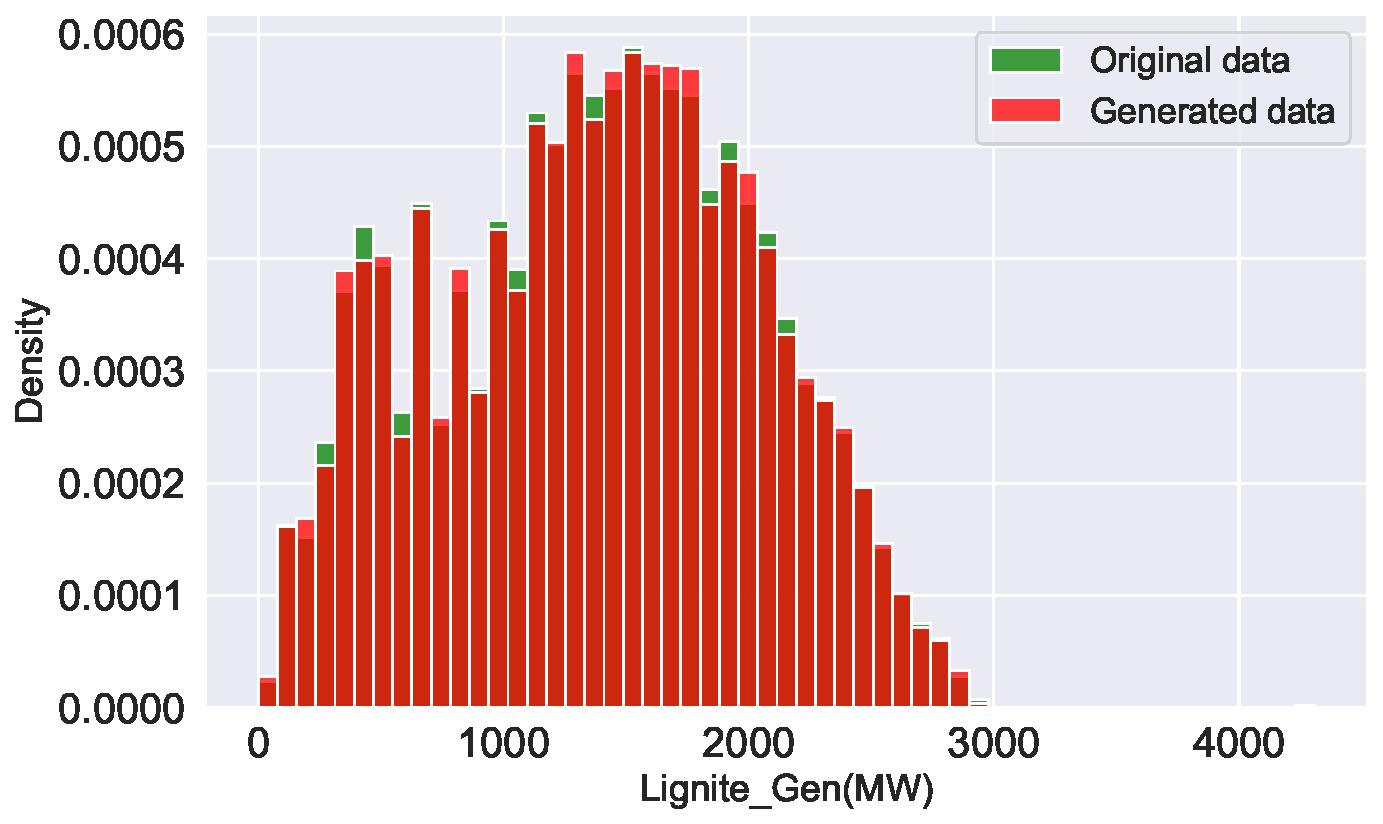
\includegraphics[width=\textwidth]{Figures/ProdCons/ProductionConsumption-Lignite-HIST.pdf}
%          \caption{Lignite\_Gen}
%          \label{fig:LginteHist}
%      \end{subfigure}
%      \begin{subfigure}[b]{0.3\textwidth}
%          \centering
%          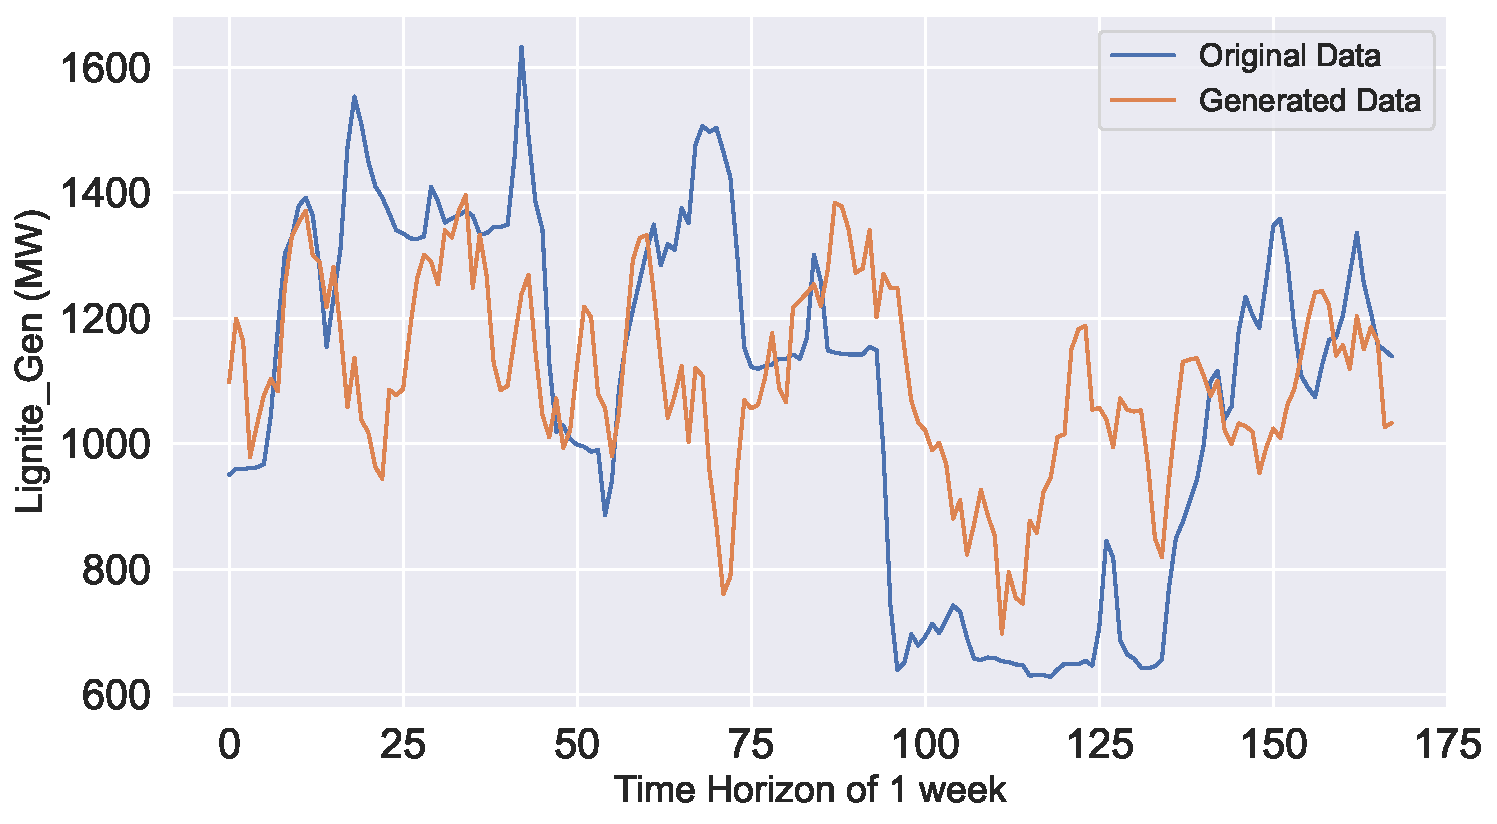
\includegraphics[width=\textwidth]{Figures/ProdCons/TimeSeries_Lignite-HIST.pdf}
%          \caption{Lignite\_Gen-Smoothed,rolling=12}
%          \label{fig:LigniteTimeSeries}
%      \end{subfigure}
     
%      \begin{subfigure}[b]{0.3\textwidth}
%          \centering
%          \includegraphics[width=\textwidth]{Figures/ProdCons/ProductionConsumption-FossilGas-HIST.pdf}
%          \caption{FossilGas\_Gen}
%          \label{fig:FossilHist}
%     \end{subfigure}
%     \begin{subfigure}[b]{0.3\textwidth}
%          \centering
%          \includegraphics[width=\textwidth]{Figures/ProdCons/TimeSeries_FossilGas-HIST-PreRolling6.pdf}
%          \caption{FossilGas\_Gen-Smoothed,rolling=6}
%          \label{fig:FossilTimeSeries}
%      \end{subfigure}
     
%      \begin{subfigure}[b]{0.3\textwidth}
%          \centering
%          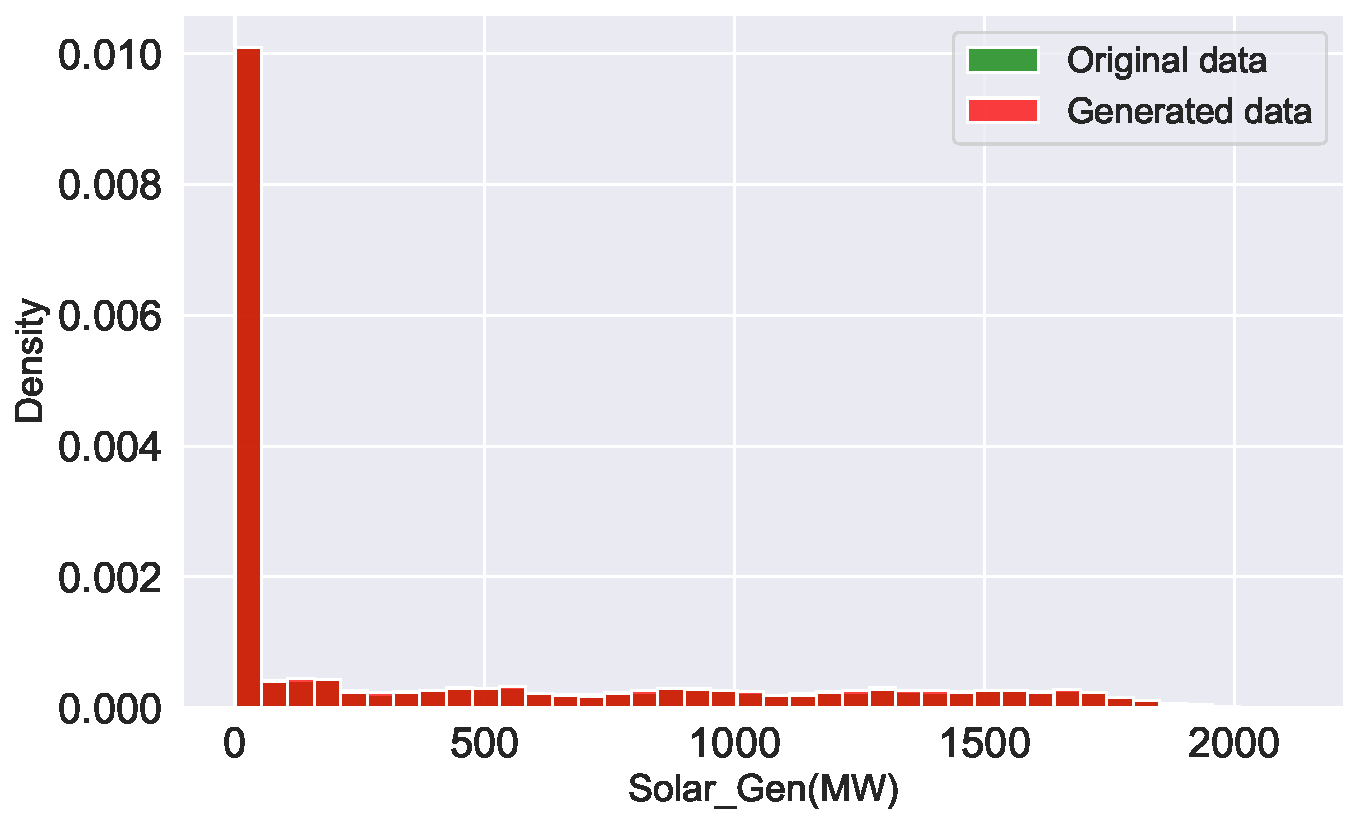
\includegraphics[width=\textwidth]{Figures/ProdCons/ProductionConsumption-Solar-HIST.pdf}
%          \caption{Solar\_Gen}
%          \label{fig:SolarHist}
%     \end{subfigure}
%     \begin{subfigure}[b]{0.3\textwidth}
%          \centering
%          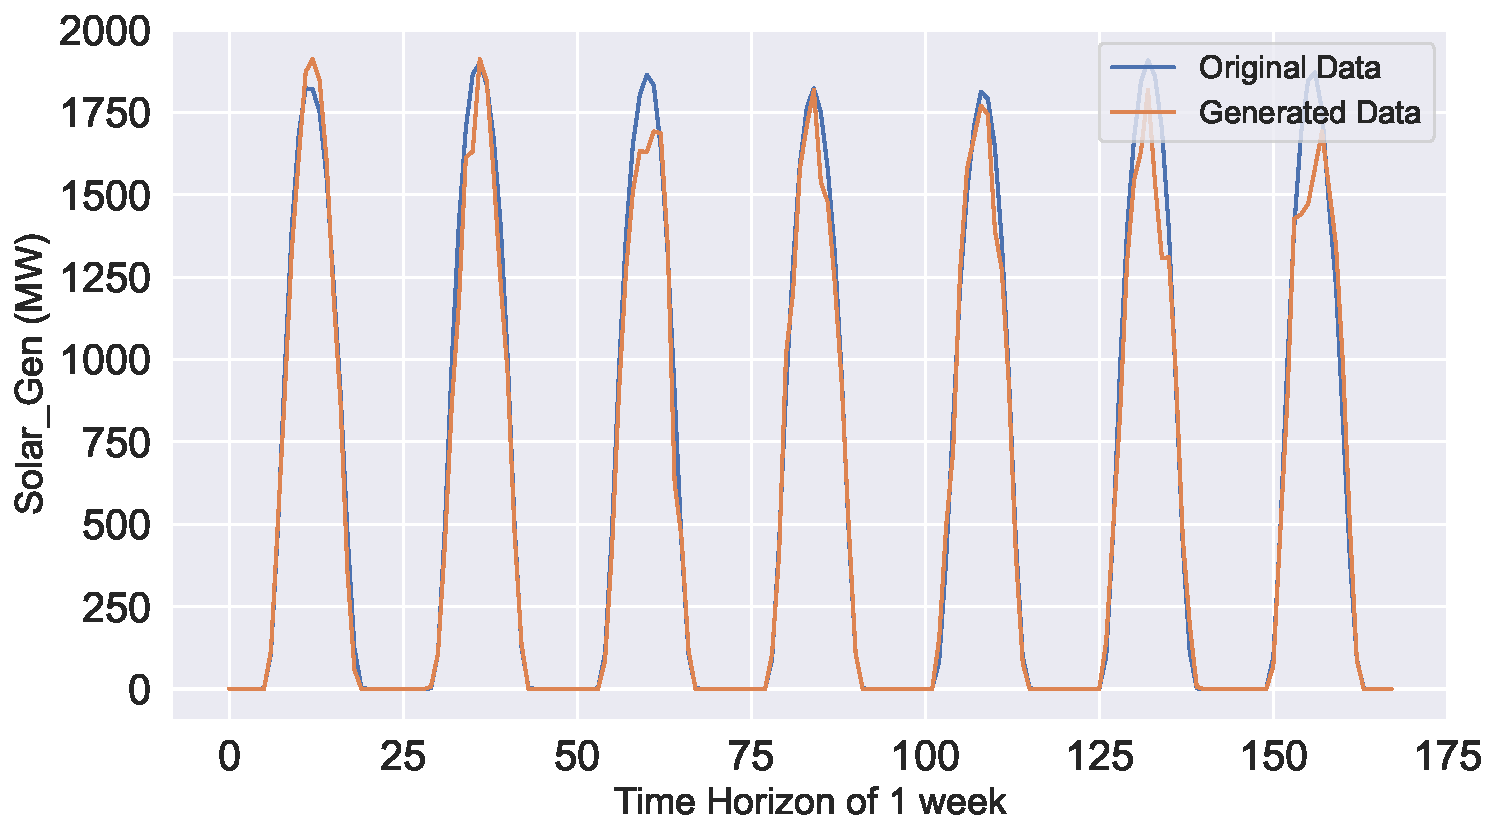
\includegraphics[width=\textwidth]{Figures/ProdCons/TimeSeries_Solar-HIST.pdf}
%          \caption{Solar\_Gen}
%          \label{fig:SolarTimeSeries}
%      \end{subfigure}
     
%      \begin{subfigure}[b]{0.3\textwidth}
%          \centering
%          \includegraphics[width=\textwidth]{Figures/ProdCons/ProductionConsumption-Wind-HIST.pdf}
%          \caption{Wind\_Gen}
%          \label{fig:WindHist}
%     \end{subfigure}
%     \begin{subfigure}[b]{0.3\textwidth}
%          \centering
%          \includegraphics[width=\textwidth]{Figures/ProdCons/TimeSeries_Wind-HIST-PreRolling12.pdf}
%          \caption{Wind\_Gen-Smoothed,rolling=12}
%          \label{fig:WindTimeSeries}
%      \end{subfigure}     
     
%       \begin{subfigure}[b]{0.3\textwidth}
%          \centering
%          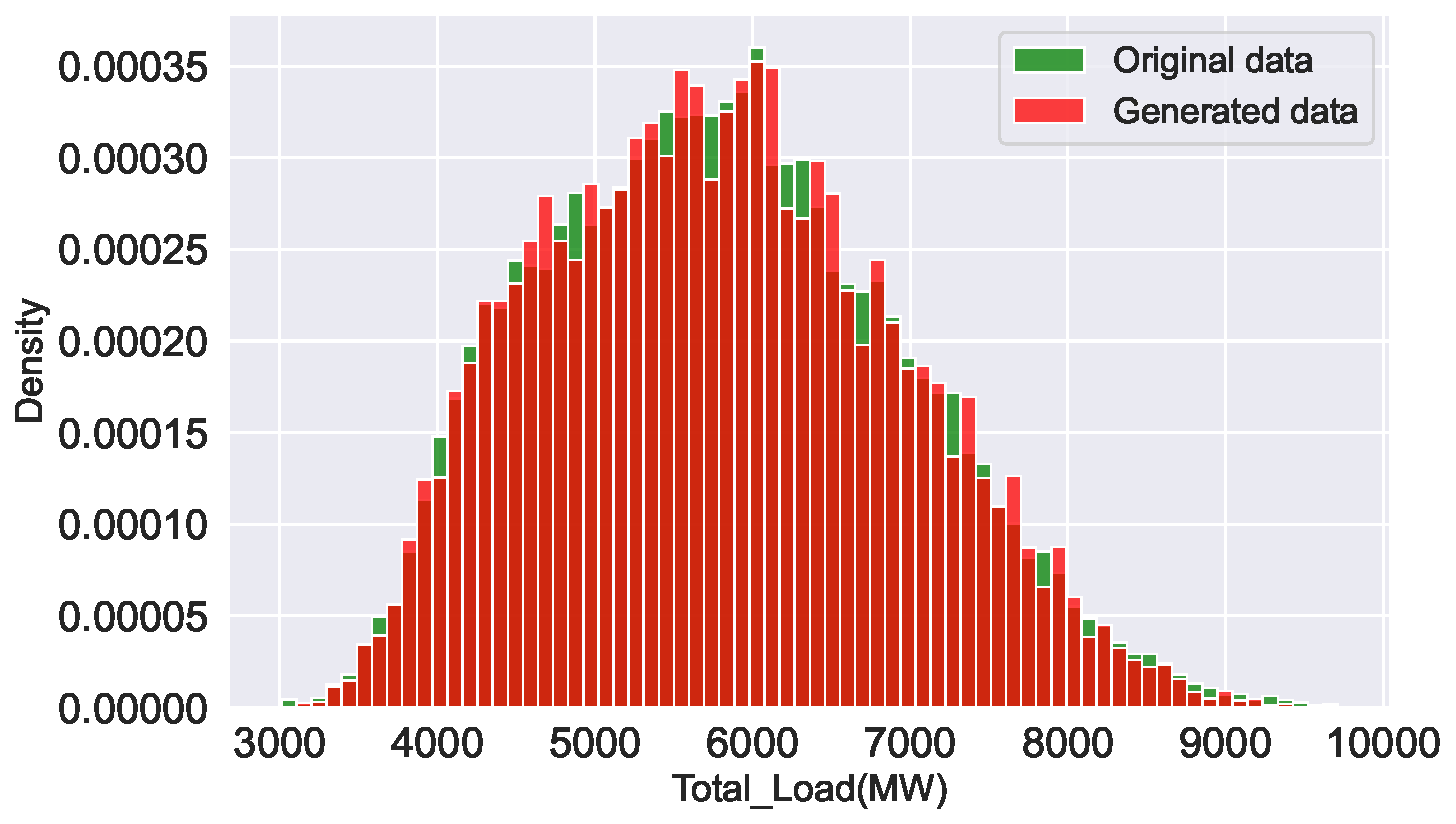
\includegraphics[width=\textwidth]{Figures/ProdCons/ProductionConsumption-TotalLoad-HIST.pdf}
%          \caption{Total\_Load}
%          \label{fig:ToalHist}
%     \end{subfigure}
%     \begin{subfigure}[b]{0.3\textwidth}
%          \centering
%          \includegraphics[width=\textwidth]{Figures/ProdCons/TimeSeries_TotalLoad-HIST-PreRolling3.pdf}
%          \caption{Total\_Load-Smoothed,rolling=12}
%          \label{fig:TotalTimeSeries}
%      \end{subfigure}    
     
%      \caption{Histograms and Time-Series of Production and Consumption Data-HIST method}
%     \label{fig:plotsProdCons}
%     \Description{The Histograms and Time-Series for each of the variables of the original and generated Energy Production and Consumption data, for HIST method.}
% \end{figure*}



\end{document}
\endinput
%%
%% End of file `sample-authordraft.tex'.
